\subsection{Proof of Risk Control}
\label{appsec:proofs}

We now briefly describe the statistical properties that lead to the guarantees underlying \gls{method}.

\paragraph{Exchangeability of sequence-level losses.}
For any fixed policy parameter, the stopping rule and terminal decision are deterministic functions of the full trajectory $X_i$. Since the calibration trajectories $(X_i,Y_i)$ are i.i.d., the induced sequence-level losses are exchangeable across samples. This allows Hoeffding's inequality to be applied to the empirical risk for each fixed candidate policy.

\paragraph{Validity of the conditional p-values.}
For the LTT procedure, the pairs $(S_i^{(j)},L_i^{(j)})$ are i.i.d. across calibration samples because each depends only on the corresponding trajectory-label pair $(X_i,Y_i)$. Conditional on the stopped index set $A_j$, the selected losses $\{L_i^{(j)}:i\in A_j\}$ remain independent. Therefore, conditional on $A_j$, the empirical conditional risk $\widehat{R}_{\mathrm{cond}}(\lambda_j)$ is the mean of $n_j$ independent $[0,1]$-valued random variables with expectation $R_{\mathrm{cond}}(\lambda_j)$ and Hoeffding's inequality yields the valid one-sided p-value \eqref{eq:hoeffding_pvalue}. Marginalizing over $A_j$ proves unconditional p-value validity.


\begin{algorithm}[H]
\caption{\gls{method}: Risk Control on Stopped Samples}
\textbf{Input:} Calibration set $\mathcal{D}_{cal}=\{(X_i,Y_i)\}_{i=1}^{n_{cal}}$, candidate grid $\Lambda=\{\lambda_1,\dots,\lambda_m\}$, target conditional risk $\alpha$, confidence level $\delta$, utility $U(\lambda)$.
\begin{algorithmic}
\FOR{$j=1,\dots,m$}
    \FOR{$i=1,\dots,n_{cal}$}
        \STATE Evaluate policy $D_{\lambda_j}$ on trajectory $X_i$ and compute stopping time
        \begin{align*}
            \tau_{\lambda_j}(X_i)=\inf\{t\in\{1,\dots,T\}:D_{\lambda_j}(X_i^t)\neq \mathrm{CONTINUE}\}
        \end{align*}
        \STATE Set
        \begin{align*}
            S_i^{(j)}=\mathbf{1}\{\tau_{\lambda_j}(X_i)<\infty\}
        \end{align*}
        \IF{$S_i^{(j)}=1$}
            \STATE Compute terminal decision
            \begin{align*}
                \hat{Y}_{\lambda_j}(X_i)=D_{\lambda_j}(X_i^{\tau_{\lambda_j}(X_i)})
            \end{align*}
            \STATE Compute loss
            \begin{align*}
                L_i^{(j)}=\mathcal{L}\bigl(\hat{Y}_{\lambda_j}(X_i),Y_i\bigr)
            \end{align*}
        \ENDIF
    \ENDFOR
    \STATE Let
    \begin{align*}
        A_j=\{i:S_i^{(j)}=1\},\qquad n_j=|A_j|
    \end{align*}
    \IF{$n_j=0$}
        \STATE Set $p_j=1$.
    \ELSE
        \STATE Compute empirical conditional risk
        \begin{align*}
            \widehat{R}_{\mathrm{cond}}(\lambda_j) = \frac{1}{n_j}\sum_{i\in A_j} L_i^{(j)}
        \end{align*}
        \STATE Compute p-value
        \begin{align*}
            p_j = \exp\!\left(-2n_j\big(\alpha-\widehat{R}_{\mathrm{cond}}(\lambda_j)\big)_+^2\right)
        \end{align*}
    \ENDIF
\ENDFOR
\STATE Apply Holm's step-down procedure to $\{p_j\}_{j=1}^m$ at level $\delta$.
\STATE Let
\begin{align*}
    \widehat{\mathcal S} = \{\lambda_j \in \Lambda : H_{0,j}\ \text{is rejected}\}
\end{align*}
\IF{$\widehat{\mathcal S}=\varnothing$}
    \STATE \textbf{return} default conservative policy or abstain.
\ELSE
    \STATE Select
    \begin{align*}
        \hat{\lambda}
        \in
        \arg\max_{\lambda_j\in\widehat{\mathcal S}} U(\lambda_j).
    \end{align*}
    \STATE \textbf{return} $\hat{\lambda}$.
\ENDIF
\end{algorithmic}\label{eq:alg_ltt}
\end{algorithm}
\newpage

\subsection{ Statistics for FastMRI Knee and Prostate Datasets}
\begin{table}[h]
\centering
\caption{Dataset statistics for \textsc{fastMRI} Knee. $N = 41,679$ slices with an approximately $80\%, 10\%, 10\%$ train/validation/test split. Patients are disjoint across partitions; the evaluated task is slice-level.}
\label{tab:fastmri_class_stats}
{%
\begin{tabular}{l|c}
\toprule
\textbf{Class Label} & \textbf{Fraction of Positive labels}  \\
\midrule
ACL Sprain      &  0.03  \\
Meniscal Tear &  0.11 \\
Abnormal        &  0.16  \\ %41679
\bottomrule
\end{tabular}
}
\end{table}


\begin{table}[h]

\centering
\caption{Clinical prostate MRI examination/volume-level split statistics. Patients are disjoint across partitions; PI-RADS positive is defined as radiologist-assigned PI-RADS $\geq 3$.}
\label{tab:prostate_dataset_stats}
{
\begin{tabular}{lcc}
\toprule
\textbf{Split} & \textbf{Total} & \textbf{Fraction of Positive Labels} \\
\midrule
Train       & 6413 & 0.48 \\
Validation  & 952  & 0.49 \\
Calibration   & 945  & 0.45 \\
Test          & 824  & 0.40 \\
\bottomrule
\end{tabular}
}
\end{table}


% =====================================================================
% Appendix: comparison with additional baselines
% Figures: figures/cifar_per_rate_lambda_test.png,
%          figures/knee_per_rate_lambda_test.png,
%          figures/prostate_per_tag_tau_test.png
% =====================================================================

\subsection{Comparison with Additional Baselines}
\label{app:baselines}

We compare \gls{method} with two more stopping baselines on all three tasks, using the same calibration and test splits and the same target level $\alpha = 0.1$ as in \cref{sec:experiments_1}. In the figures, \emph{LTT} denotes \gls{method}. Each figure follows the same layout. The \textbf{left panel} shows the cumulative fraction of test samples on which acquisition has stopped. The \textbf{remaining panels} show the risk among the stopped samples, and the horizontal line marks the target.

\paragraph{Baselines.}
\textbf{Operating Point Method:} At each acquisition time, we select a threshold on the calibration set to target empirical task-specific risk $\alpha$ across all calibration samples.
\textbf{Selective Inference:} At each acquisition time, we similarly select a threshold on the calibration set, but evaluate empirical risk only among the samples selected for early stopping. The risk is misclassification on \textsc{cifar}-10 and class-conditional \textsc{fnr} for the MRI tasks. Both baselines use the same calibration and test splits as \gls{method}, with nominal target $\alpha=0.1$. Neither empirical threshold-selection procedure, as implemented here, provides the finite-sample risk certificate of \gls{method}.

% ---------------------------------------------------------------------
\paragraph{CIFAR-10.}
\Cref{fig:app_baselines_cifar} reports the accuracy among stopped samples, with target $1-\alpha = 0.9$. The Operating Point Method stops the most samples (from about $25\%$ at a $10\%$ sampling rate to about $90\%$ at full acquisition), but its stopped-sample accuracy stays between $0.68$ and $0.74$, far below the target. Selective Inference stops no samples at a $10\%$ sampling rate and reaches $0.92$ accuracy at $20\%$. From $30\%$ onward its accuracy falls below the target, ending near $0.84$. \gls{method} stops fewer samples (about $52\%$ by full acquisition). Its stopped-sample accuracy is above $0.9$ from a $40\%$ sampling rate onward and ends at about $0.905$. At the two earliest rates, \gls{method}'s cumulative accuracy is below the target ($0.83$ and $0.88$) while only $7$--$16\%$ of samples have stopped. This does not contradict the policy-level guarantee, which controls conditional risk among all eventually stopped samples, rather than simultaneously for each intermediate cumulative stopping set $\{\tau_\lambda \leq t\}$. Checkpoint-level accuracies are therefore empirical diagnostics, not separately certified bounds. By the final acquisition stage, stopped-sample accuracy reaches about $0.905$, consistent with the target.

\begin{figure}[H]
    \centering
    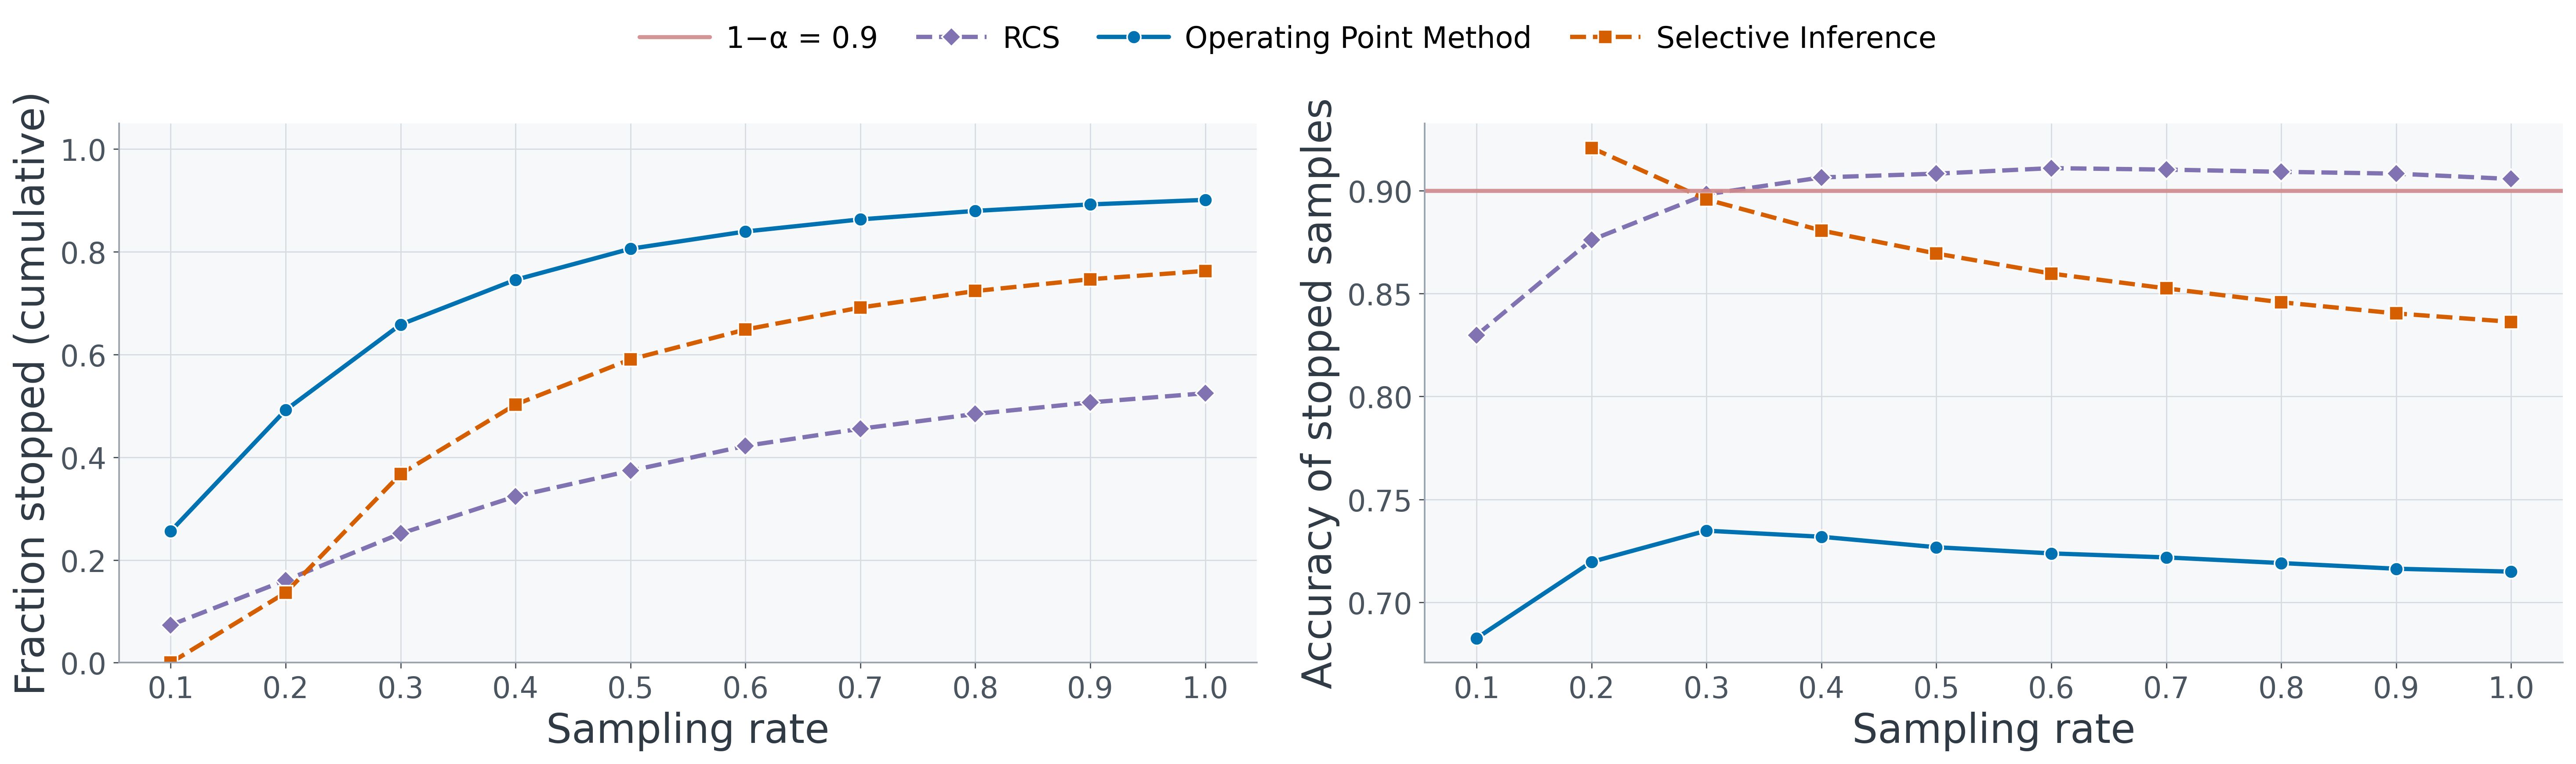
\includegraphics[width=\linewidth]{figures/cifar_per_rate_lambda_test.png}
    \caption{\textbf{Baseline comparison on \textsc{cifar}-10 ($\alpha = 0.1$).}
    \textbf{Left:} cumulative fraction of samples stopped against sampling rate.
    \textbf{Right:} accuracy among stopped samples; the horizontal line marks the target $1-\alpha = 0.9$.}
    \label{fig:app_baselines_cifar}
\end{figure}

% ---------------------------------------------------------------------
\paragraph{FastMRI knee.}
\Cref{fig:app_baselines_knee} reports the class-conditional \textsc{fnr} among stopped positives, separately for \textsc{acl} tear and meniscus tear. The Operating Point Method stops $45$--$81\%$ of slices, but its \textsc{fnr} is $0.19$--$0.23$ for \textsc{acl} and $0.25$--$0.28$ for meniscus tears, two to three times the target. Selective Inference stays within the target ($\textsc{fnr} \le 0.03$ for \textsc{acl} and $\le 0.065$ for meniscus) but stops no slices at the $5\%$ and $8\%$ sampling rates. From $12.5\%$ onward it stops more slices than \gls{method} (up to $57\%$ at $25\%$). \gls{method} is the only method that stops slices at the lowest rates while staying within the target. It stops $13\%$ of slices at $5\%$ sampling and $37\%$ at $25\%$, with an \textsc{acl} \textsc{fnr} of $0$ and a meniscus \textsc{fnr} of at most $0.012$.

\begin{figure}[H]
    \centering
    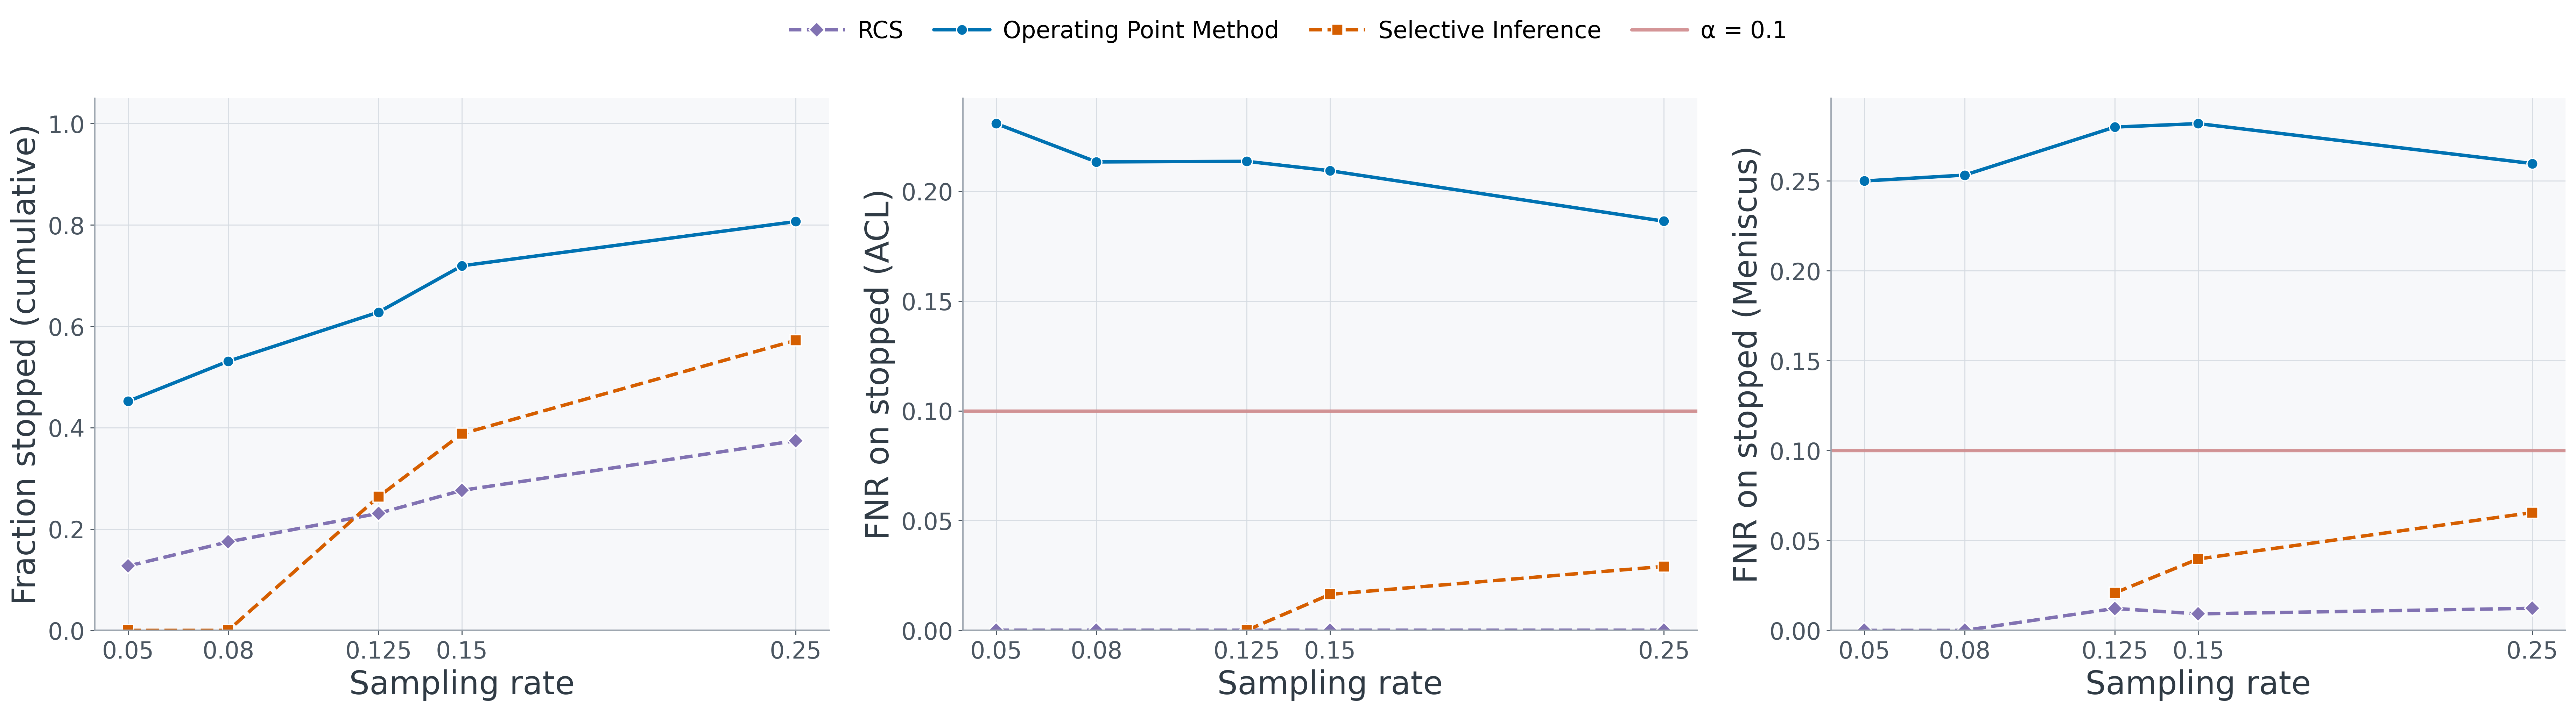
\includegraphics[width=\linewidth]{figures/knee_per_rate_lambda_test.png}
    \caption{\textbf{Baseline comparison on \textsc{fastMRI} knee ($\alpha = 0.1$).}
    \textbf{Left:} cumulative fraction of slices stopped against sampling rate.
    \textbf{Center:} \textsc{fnr} among stopped \textsc{acl}-tear positives.
    \textbf{Right:} \textsc{fnr} among stopped meniscus-tear positives.
    The horizontal line marks the target $\alpha = 0.1$.}
    \label{fig:app_baselines_knee}
\end{figure}

% ---------------------------------------------------------------------
\paragraph{Clinical prostate MRI.}
\Cref{fig:app_baselines_prostate} reports the \textsc{fnr} among stopped PI-RADS-positive exams across the $15$ scanner-ordered checkpoints of \cref{sec:experiments_1}. The tag \texttt{b50\_$i$\_b1000\_$j$} means that $i$ averages at $b=50$ and $j$ averages at $b=1000$ have been acquired. The Operating Point Method stops $55$--$76\%$ of exams with an \textsc{fnr} of $0.14$--$0.17$. Selective Inference stops $48$--$68\%$ of exams, but its \textsc{fnr} ($0.105$--$0.14$) is above the target at every checkpoint. \gls{method} stops fewer exams ($36$--$53\%$) and keeps the \textsc{fnr} between $0.026$ and $0.064$, below the target at every checkpoint.

\begin{figure}[H]
    \centering
    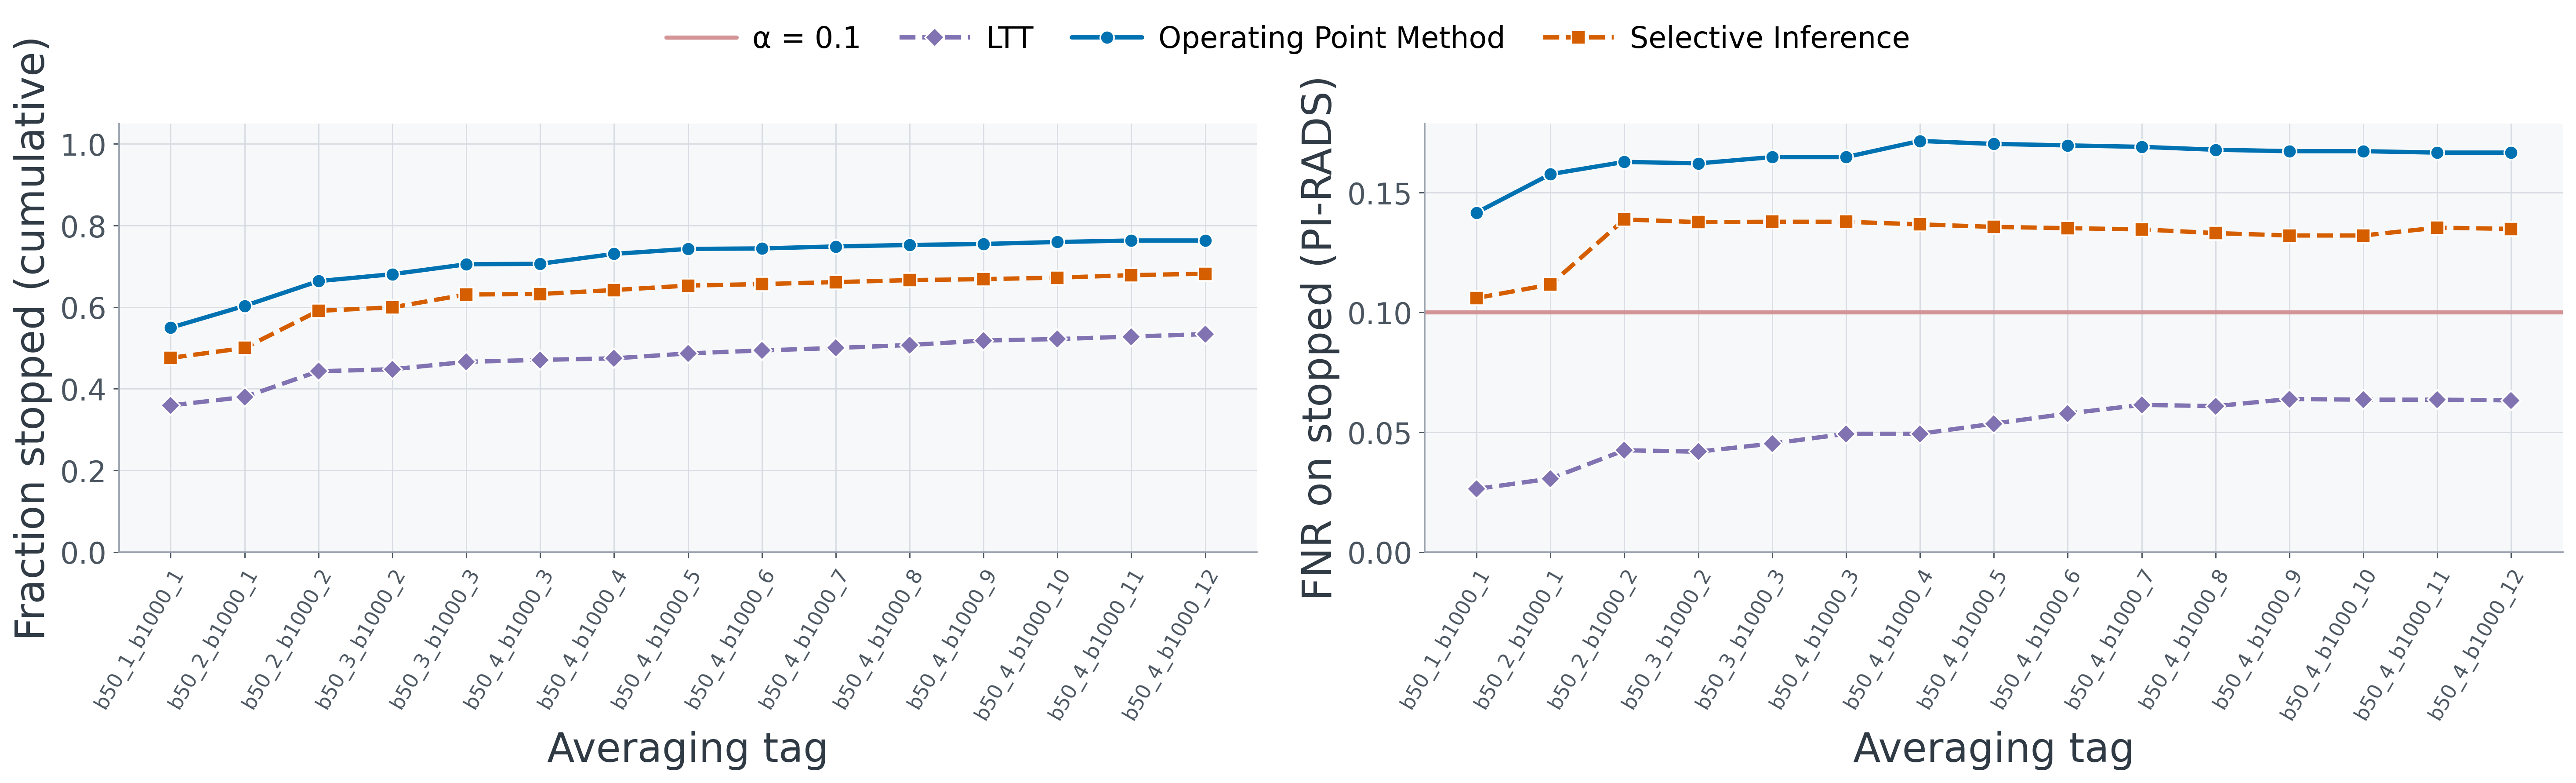
\includegraphics[width=\linewidth]{figures/prostate_per_tag_tau_test.png}
    \caption{\textbf{Baseline comparison on clinical prostate \textsc{mri} ($\alpha = 0.1$).}
    \textbf{Left:} cumulative fraction of exams stopped at each DWI checkpoint.
    \textbf{Right:} \textsc{fnr} among stopped PI-RADS-positive exams; the horizontal line marks the target $\alpha = 0.1$.
    Tags \texttt{b50\_$i$\_b1000\_$j$} give the number of $b=50$ and $b=1000$ averages acquired so far.}
    \label{fig:app_baselines_prostate}
\end{figure}

% ---------------------------------------------------------------------
\paragraph{Summary.}
The Operating Point Method stops the most samples on every task but exceeds the target risk on all three. Selective Inference stays within the target on knee but exceeds it on \textsc{cifar}-10 (from a $30\%$ sampling rate onward) and on prostate (at every checkpoint). At the final acquisition horizon, \gls{method} meets the empirical stopped-cohort risk target in all three tasks, while the two earliest \textsc{cifar}-10 checkpoint accuracies fall below the target. These intermediate measurements are not separately certified. \gls{method} generally stops fewer samples than the baselines, although the relative efficiency changes with acquisition time.
% =====================================================================
% Appendix: ablations on delta, lambda-grid density, calibration-set size
% Figures: figures/ablation_cifar_all.png,
%          figures/ablation_knee_all.png,
%          figures/ablation_prostate_all.png
% =====================================================================

\subsection{Sensitivity to Calibration Hyperparameters}
\label{app:ablations}

\gls{method} has three calibration hyper-parameters: the significance level $\delta$ of the Holm correction, the number of candidate values in the grid $\Lambda$, and the calibration set size $n_{\text{cal}}$. We vary one at a time and hold the other two at their defaults, with $\alpha = 0.1$ throughout. \Cref{fig:app_ablation_cifar,fig:app_ablation_knee,fig:app_ablation_prostate} share one layout. Row~(a) varies $\delta$, row~(b) varies the grid size, and row~(c) varies $n_{\text{cal}}$. Within each row, the left panel shows the cumulative fraction of test samples stopped and the remaining panels show the risk among stopped samples. The thick black curve is the default setting. Each legend entry gives the selected parameter $\hat\lambda$, or states that no $\lambda$ was certified, in which case \gls{method} stops no samples and every sample is fully acquired. Settings that select the same $\hat\lambda$ give identical curves and share one legend entry.

\paragraph{CIFAR-10.}
The defaults are $\delta = 0.05$, a grid of $101$ values and $n_{\text{cal}} = 4800$, which select $\hat\lambda = 0.94$ (\cref{fig:app_ablation_cifar}). For this policy family, a larger $\lambda$ is a stricter confidence threshold.
\textbf{(a)} The result barely depends on $\delta$. $\delta \in \{0.05, 0.1, 0.2\}$ all select $\hat\lambda = 0.94$. The stricter $\delta \in \{0.01, 0.025\}$ select $\hat\lambda = 0.95$, which stops slightly fewer samples ($50\%$ vs.\ $52\%$ at full acquisition) with slightly higher final accuracy ($0.914$ vs.\ $0.906$).
\textbf{(b)} Grids of $21$ to $501$ values select $\hat\lambda$ between $0.94$ and $0.95$, with nearly identical curves. The coarsest grid ($11$ values, step $0.1$) certifies no $\lambda$, because it contains no value between the unsafe region and the trivially conservative end of the grid.
\textbf{(c)} The calibration set size matters most. With $n_{\text{cal}} \in \{250, 500, 1000\}$, no $\lambda$ is certified. With $n_{\text{cal}} = 2000$, \gls{method} certifies the more conservative $\hat\lambda = 0.98$. This stops $39\%$ of samples by full acquisition (vs.\ $52\%$ at the default), with final accuracy $0.94$.
In every certified setting, the stopped-sample accuracy is above $0.9$ from a $30$--$40\%$ sampling rate onward. At the two earliest rates it is below the target, as in \cref{app:baselines}.

\begin{figure}[H]
    \centering
    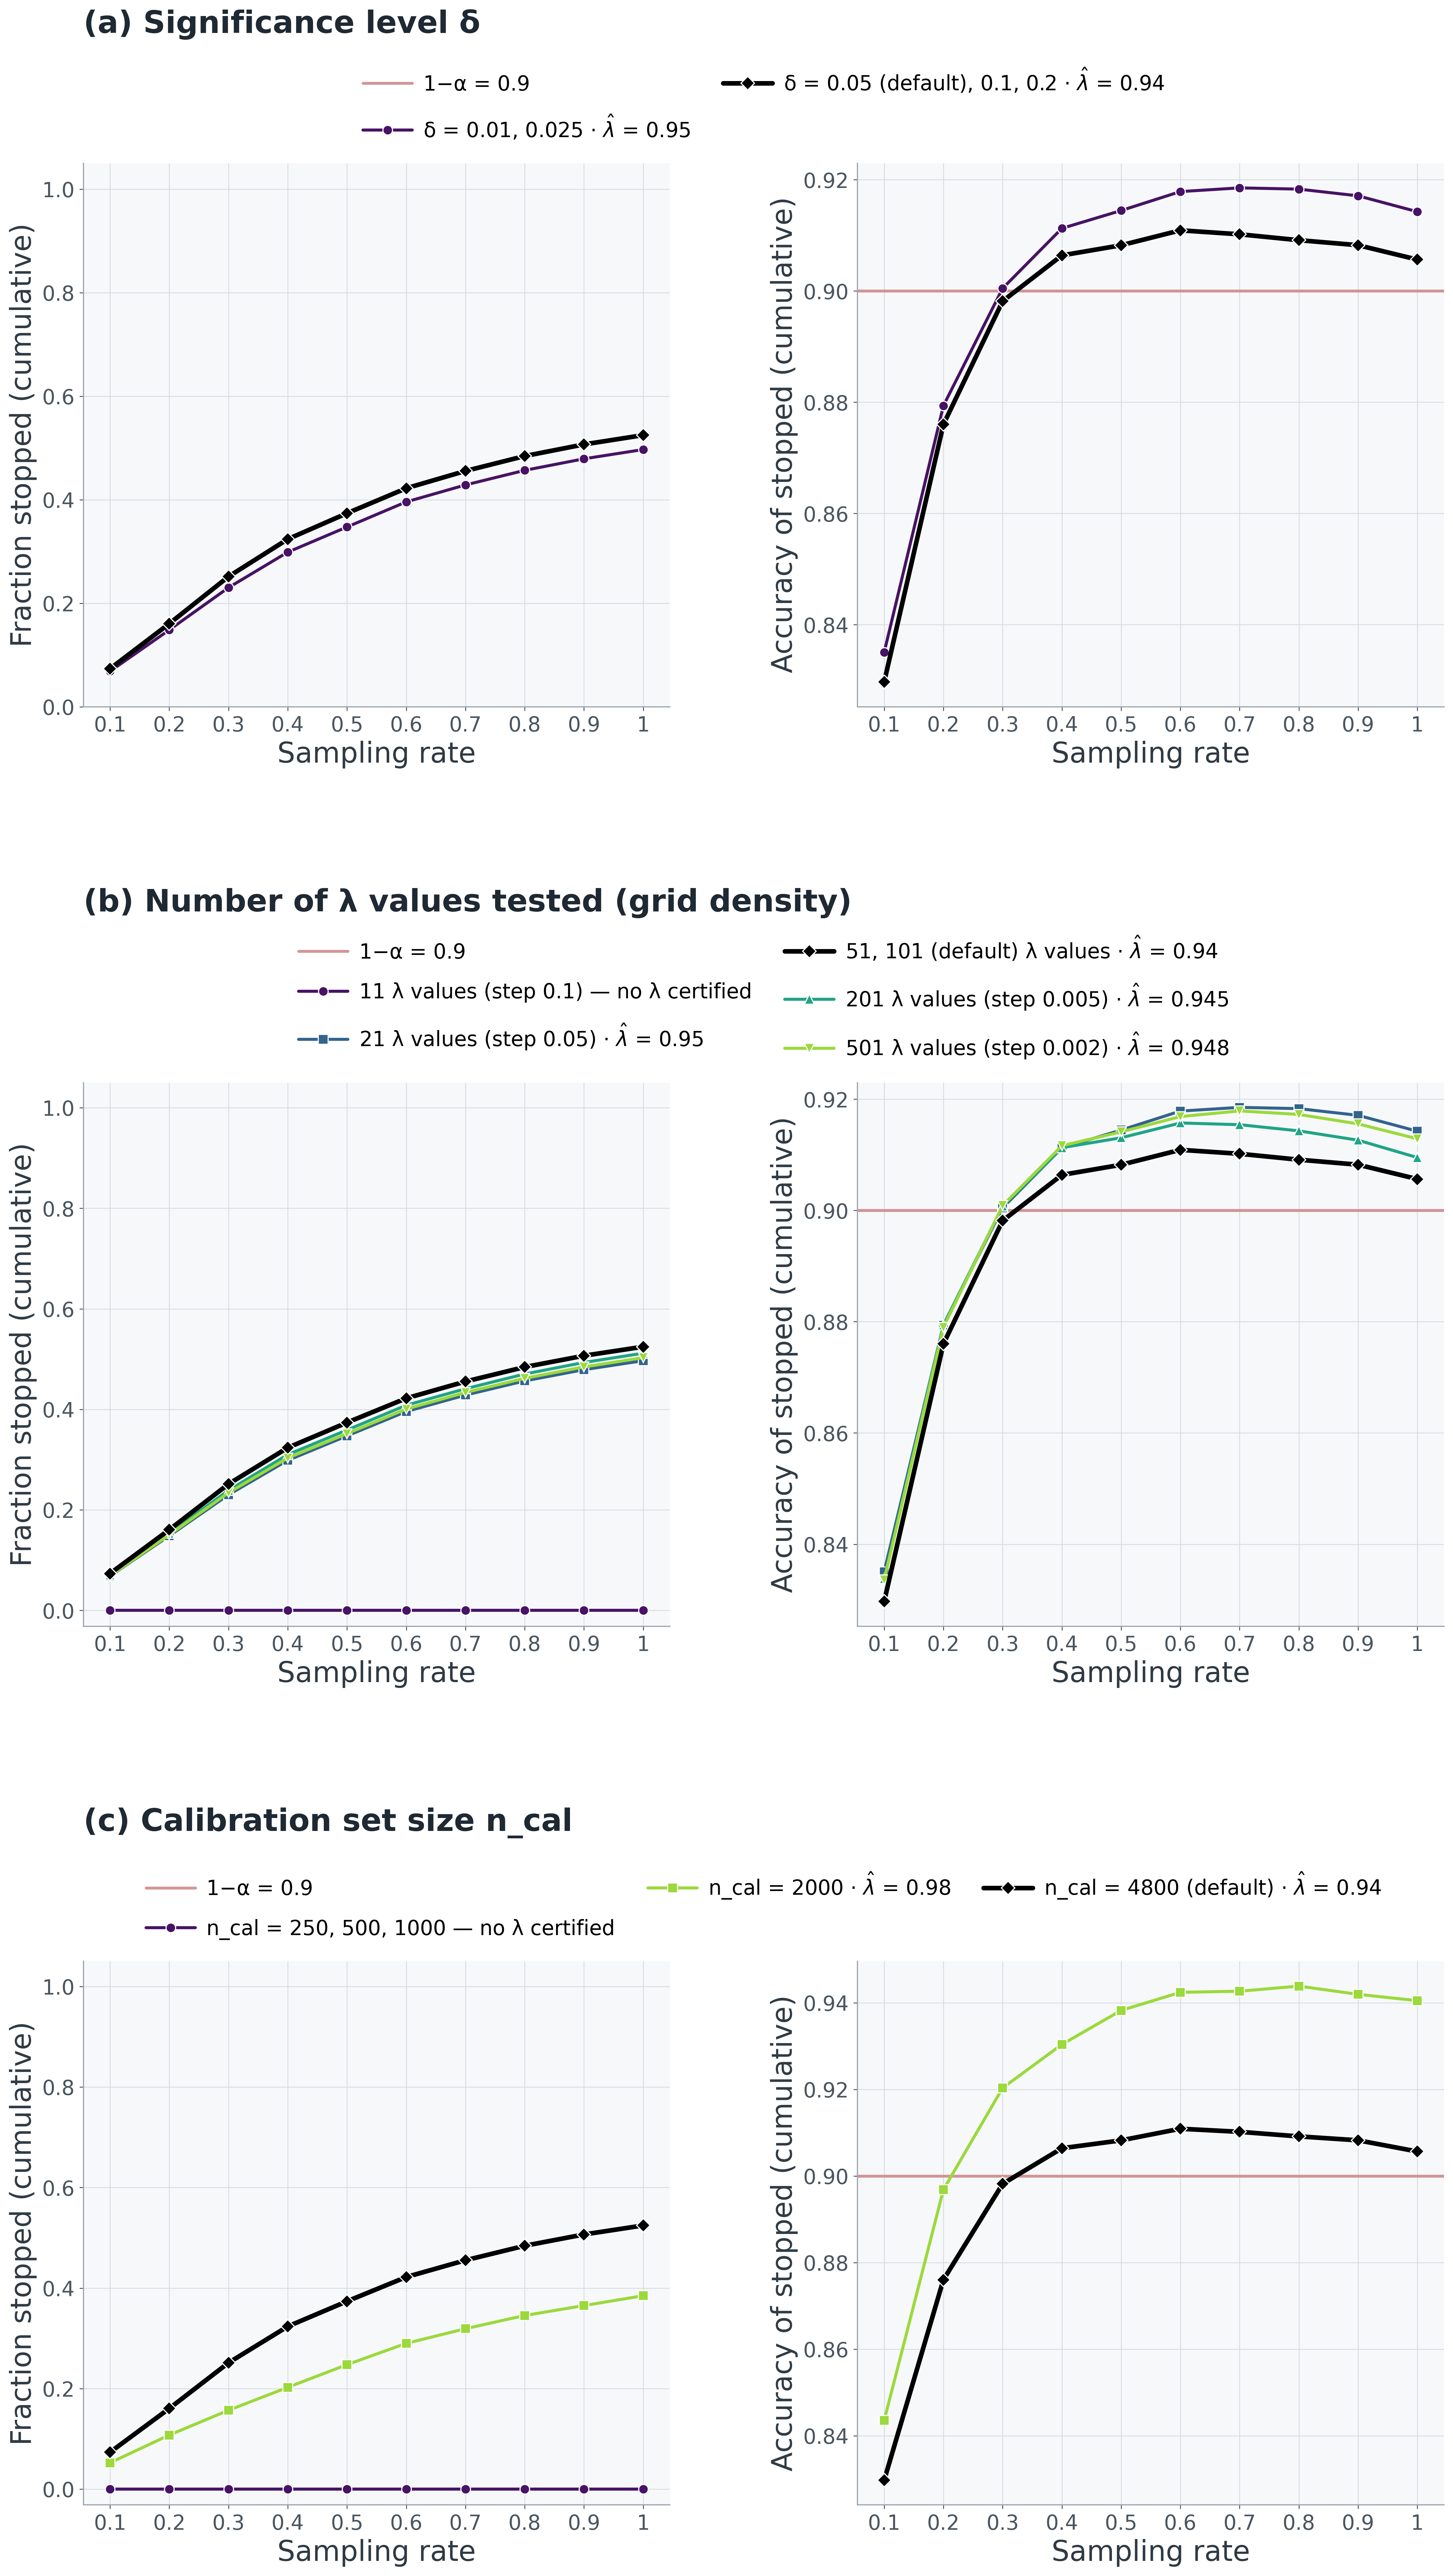
\includegraphics[width=\linewidth,height=0.8\textheight,keepaspectratio]{figures/ablation_cifar_all.png}
    \caption{\textbf{Hyperparameter sensitivity on \textsc{cifar}-10 ($\alpha = 0.1$).}
    \textbf{(a)} Significance level $\delta$.
    \textbf{(b)} Number of $\lambda$ values in the grid.
    \textbf{(c)} Calibration set size $n_{\text{cal}}$.
    Left: cumulative fraction of samples stopped. Right: accuracy among stopped samples; the horizontal line marks $1-\alpha = 0.9$. The thick black curve is the default setting.}
    \label{fig:app_ablation_cifar}
\end{figure}

% ---------------------------------------------------------------------
\paragraph{FastMRI knee.}
The defaults are $\delta = 0.1$, a grid of $15$ values and $n_{\text{cal}} = 6180$, which select $\hat\lambda = 0.4286$ (\cref{fig:app_ablation_knee}). For the ambiguity bands, a larger $\lambda$ is a narrower band and more aggressive stopping.
\textbf{(a)} $\delta = 0.01$ certifies no $\lambda$. The other levels select $\hat\lambda$ between $0.36$ and $0.5$. Every resulting policy keeps both pathology-specific \textsc{fnr}s at or below $0.044$, well under the target. The selected thresholds differ across evaluated significance levels; these values describe the reported sensitivity sweep and do not establish a general monotone relationship between $\delta$ and the selected threshold.
\textbf{(b)} Grid sizes from $3$ to $113$ select $\hat\lambda$ between $0.43$ and $0.51$. The stopped fraction at a $25\%$ sampling rate ranges from $37\%$ to $46\%$, and the \textsc{fnr} stays at or below $0.05$ for both pathologies.
\textbf{(c)} Only the full calibration set certifies a $\lambda$. With $n_{\text{cal}} \in \{500, 1000, 2000, 4000\}$, no $\lambda$ is certified. These subsets contain only $12$--$93$ \textsc{acl}-tear positives, too few to certify an \textsc{fnr} bound for this rare pathology. \gls{method} then certifies no early-stopping candidate and defers every slice to full acquisition.

\begin{figure}[H]
    \centering
    \includegraphics[width=\linewidth,height=0.8\textheight,keepaspectratio]{figures/ablation_knee_all.png}
    \caption{\textbf{Hyperparameter sensitivity on \textsc{fastMRI} knee ($\alpha = 0.1$).}
    \textbf{(a)} Significance level $\delta$.
    \textbf{(b)} Number of $\lambda$ values in the grid.
    \textbf{(c)} Calibration set size $n_{\text{cal}}$; the legend gives the number of \textsc{acl}-tear and meniscus-tear positives in each calibration set.
    Left: cumulative fraction of slices stopped. Center/Right: \textsc{fnr} among stopped \textsc{acl}-tear and meniscus-tear positives; the horizontal line marks $\alpha = 0.1$. The thick black curve is the default setting.}
    \label{fig:app_ablation_knee}
\end{figure}

% ---------------------------------------------------------------------
\paragraph{Clinical prostate MRI.}
The defaults are $\delta = 0.1$, a grid of $51$ values and $n_{\text{cal}} = 745$, which select $\hat\lambda = 0.58$ (\cref{fig:app_ablation_prostate}). Of the $945$ examinations in the calibration partition reported in \cref{tab:prostate_dataset_stats}, $745$ are used for risk calibration. The remaining $200$ examinations were unused in these experiments, including for ambiguity-band estimation.
\textbf{(a)} $\delta \in \{0.01, 0.025, 0.05, 0.1\}$ all select $\hat\lambda = 0.58$. $\delta = 0.2$ selects $\hat\lambda = 0.6$, which stops about $4$ percentage points more exams and has an \textsc{fnr} of at most $0.077$.
\textbf{(b)} Grid sizes from $6$ to $201$ select $\hat\lambda$ between $0.58$ and $0.6$. The curves differ by a few percentage points, and every \textsc{fnr} stays below $0.08$.
\textbf{(c)} With $n_{\text{cal}} \in \{100, 200\}$ ($41$ and $84$ PI-RADS-positive exams), no $\lambda$ is certified. From $n_{\text{cal}} = 400$ ($168$ positives) upward, the selection is stable at $\hat\lambda = 0.58$.

\begin{figure}[H]
    \centering
    \includegraphics[width=\linewidth,height=0.8\textheight,keepaspectratio]{figures/ablation_prostate_all.png}
    \caption{\textbf{Hyperparameter sensitivity on clinical prostate \textsc{mri} ($\alpha = 0.1$).}
    \textbf{(a)} Significance level $\delta$.
    \textbf{(b)} Number of $\lambda$ values in the grid.
    \textbf{(c)} Calibration set size $n_{\text{cal}}$; the legend gives the number of PI-RADS-positive exams in each calibration set.
    Left: cumulative fraction of exams stopped at each DWI checkpoint. Right: \textsc{fnr} among stopped PI-RADS-positive exams; the horizontal line marks $\alpha = 0.1$. The thick black curve is the default setting.}
    \label{fig:app_ablation_prostate}
\end{figure}

% ---------------------------------------------------------------------
\paragraph{Summary.}
\gls{method} is insensitive to $\delta$ and to the grid size over a wide range. Changing either moves $\hat\lambda$ only slightly, and the stopped-sample risk stays below the target in every certified setting, except at the two earliest \textsc{cifar}-10 rates. A very coarse grid can miss the safe region entirely (\textsc{cifar}-10, $11$ values). The calibration set size is the main limit. What matters is the number of calibration samples in the class whose error rate is controlled. For prostate, $84$ PI-RADS positives were too few and $168$ were enough. For knee, $93$ \textsc{acl}-tear positives were too few and the full set's $155$ were enough. Below that, \gls{method} certifies no rule and defers to full acquisition rather than returning an unsafe one.

% \begin{figure}[ht]
%     \centering
%     \begin{minipage}{0.48\textwidth}
%         \centering
%         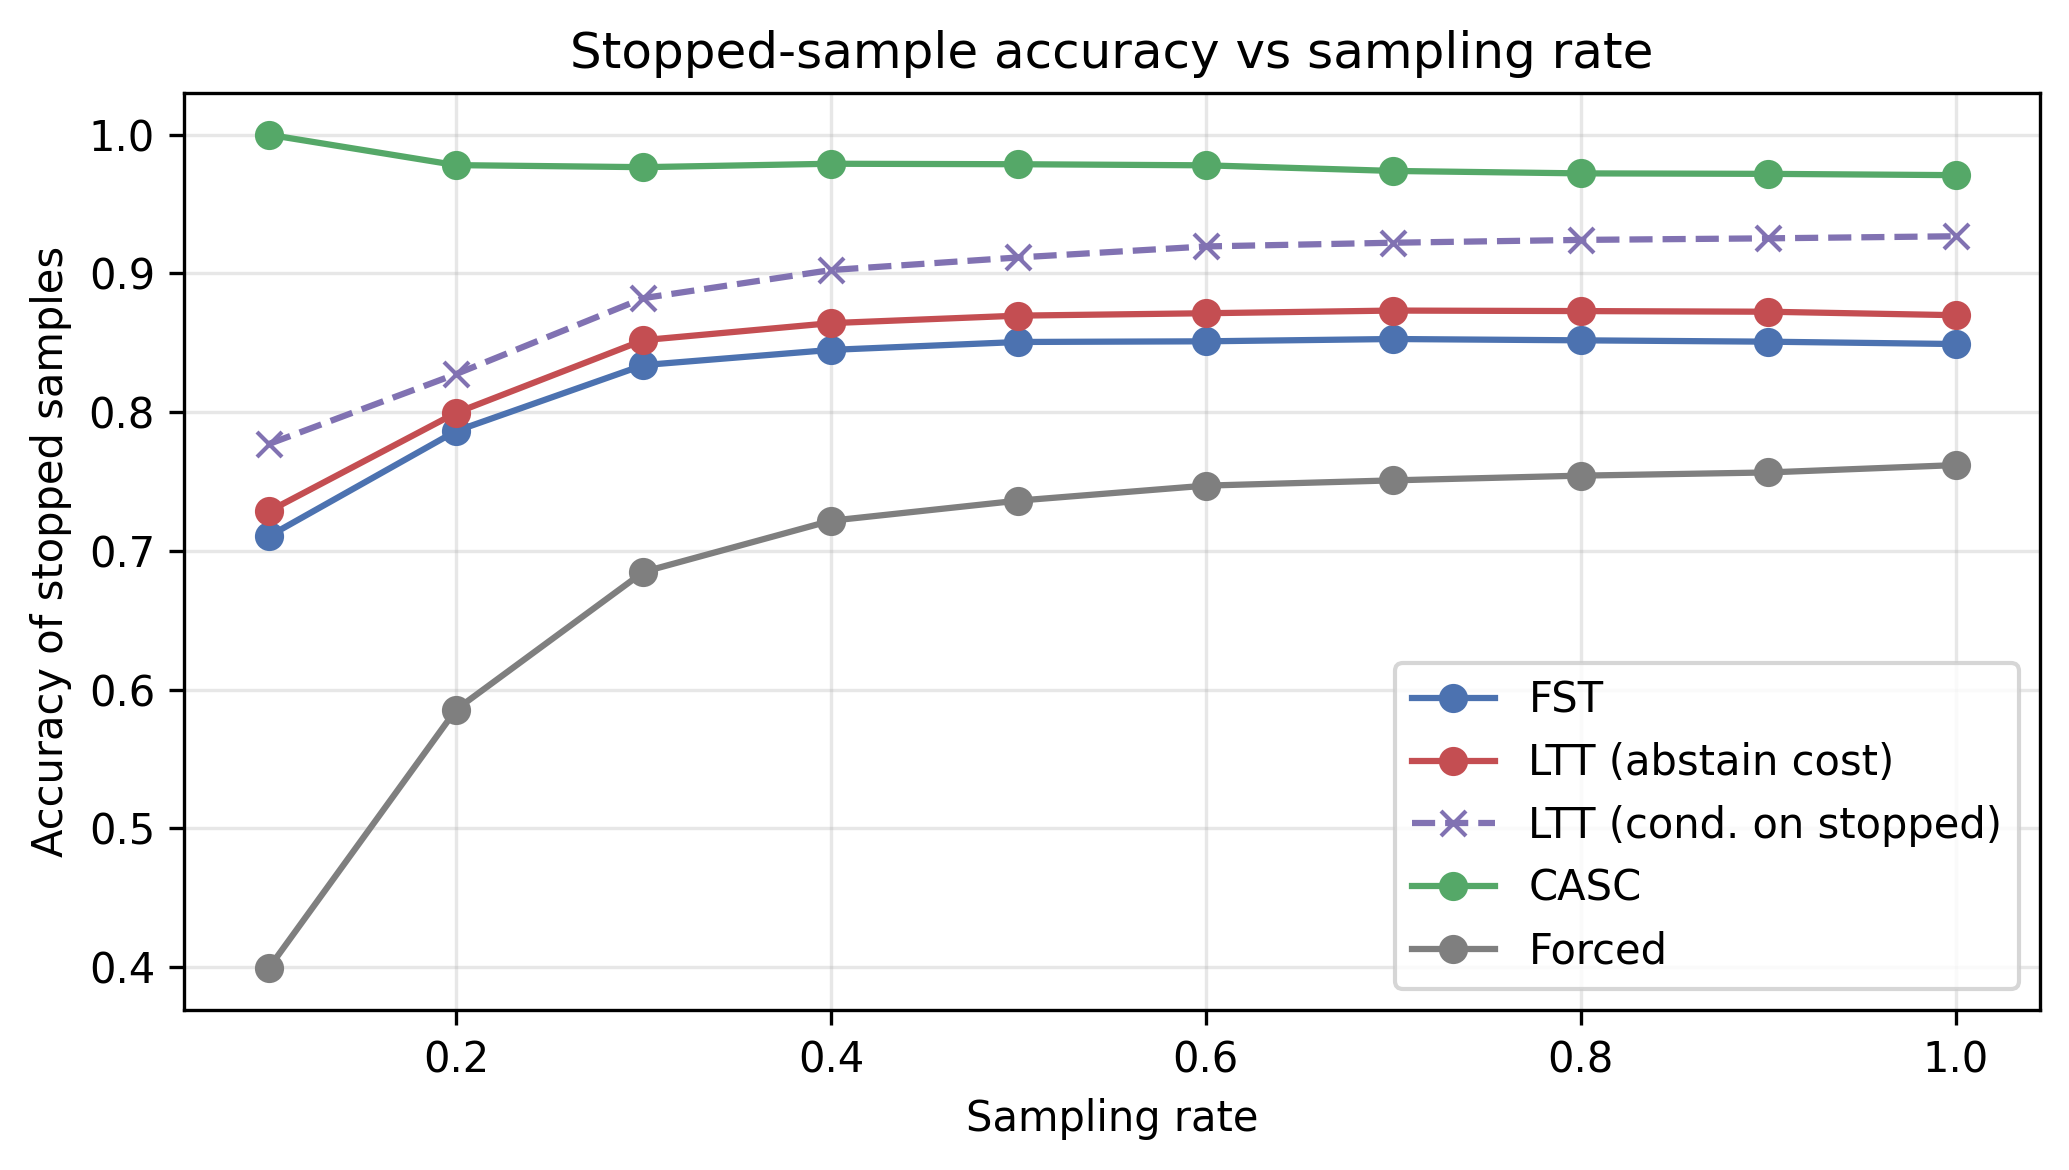
\includegraphics[width=\linewidth]{figures/cifar10_compare_stopped_accuracy_vs_sampling_rate_max_score.png}
%         \caption*{(a) \textbf{CIFAR-10} : Accuracy among stopped samples against sampling rate}
%     \end{minipage}\hfill
%     \begin{minipage}{0.48\textwidth}
%         \centering
%         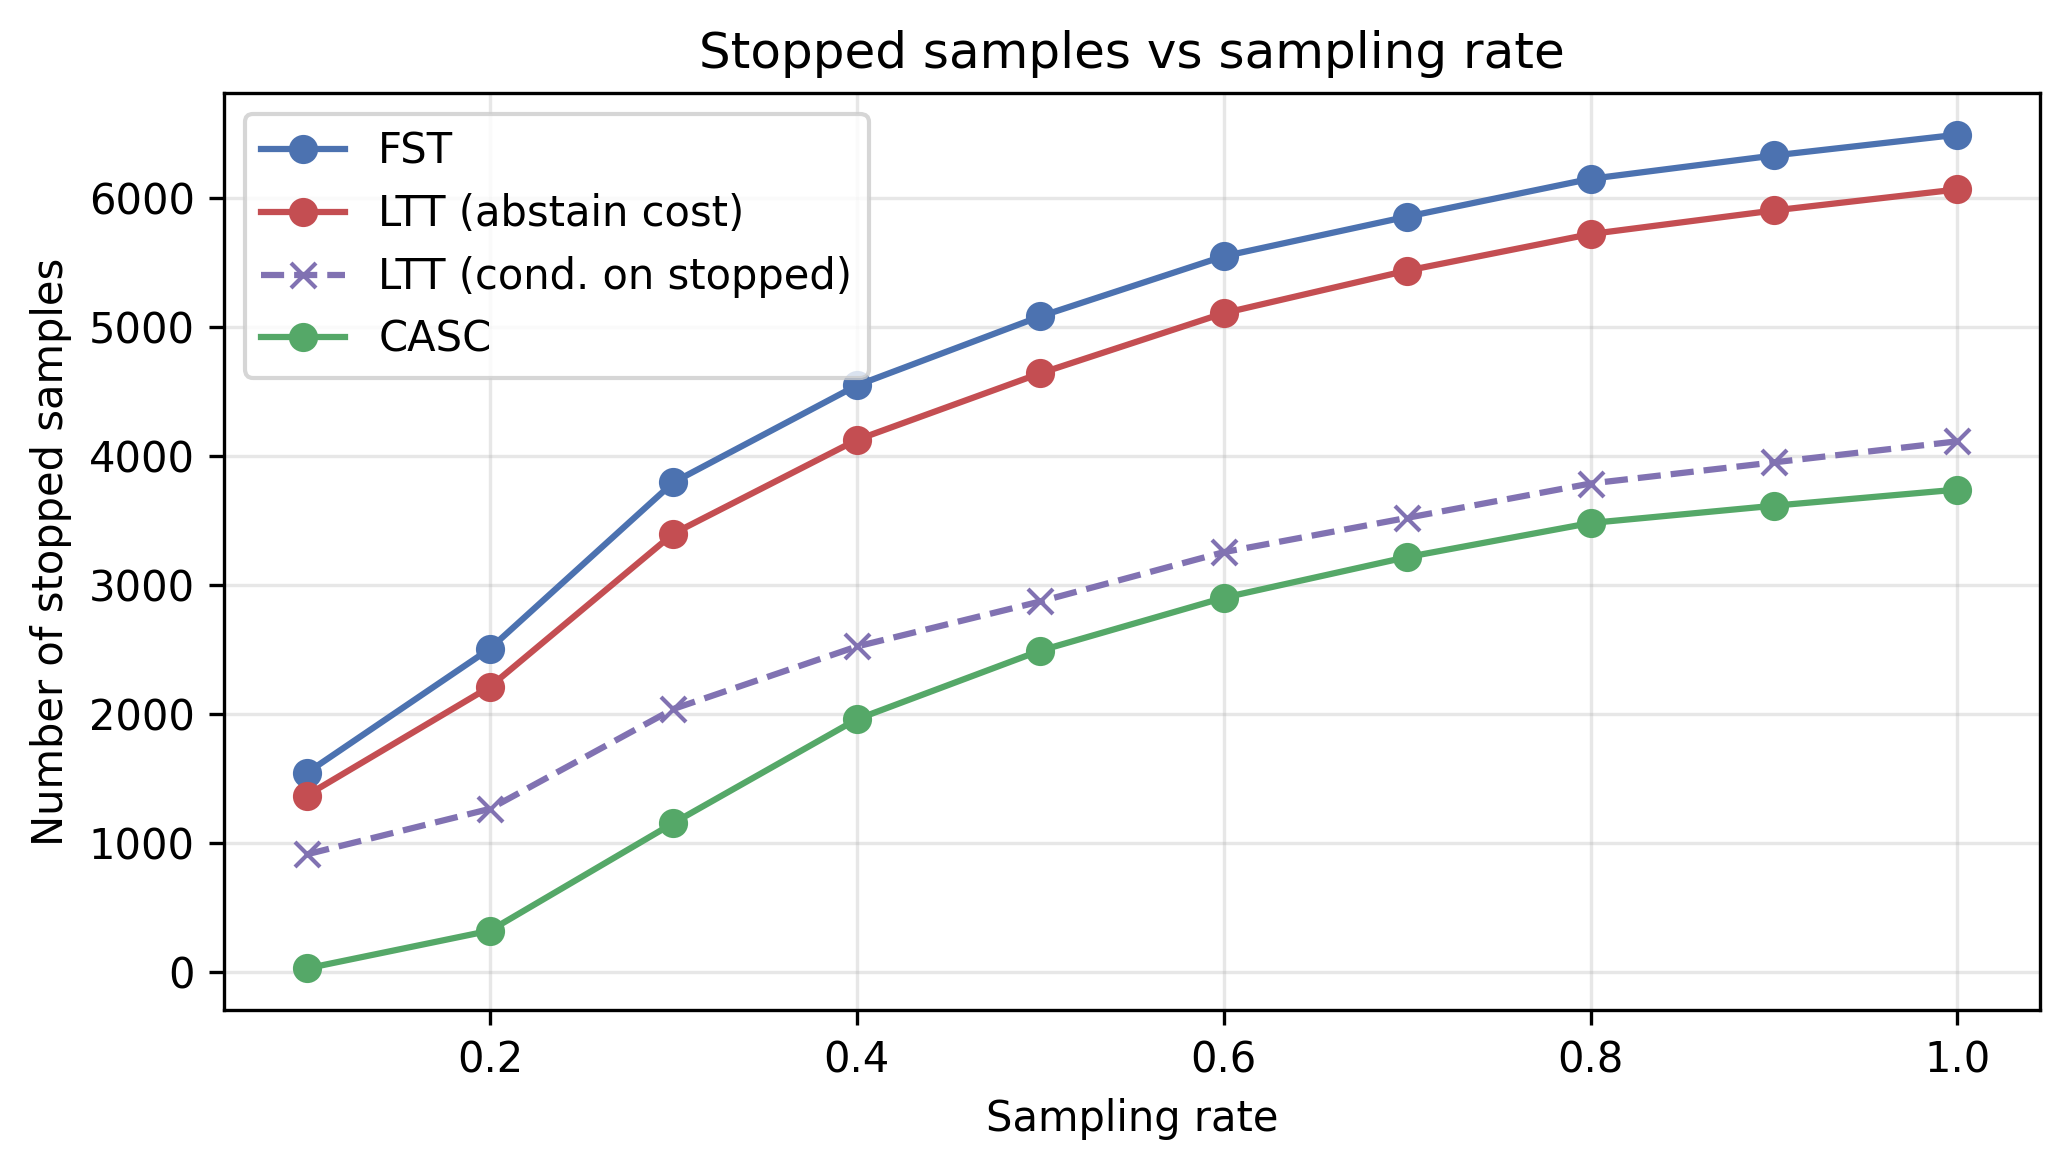
\includegraphics[width=\linewidth]{figures/cifar10_compare_stopped_vs_sampling_rate_max_score.png}
%         \caption*{\textbf{CIFAR-10} : Fraction of stopped samples against sampling rate}
%     \end{minipage}
%     \caption{CIFAR-10  Results}
%     \label{fig:two-plots}
% \end{figure}

% \begin{figure}[ht]
%     \centering
%     \begin{minipage}{0.48\textwidth}
%         \centering
%         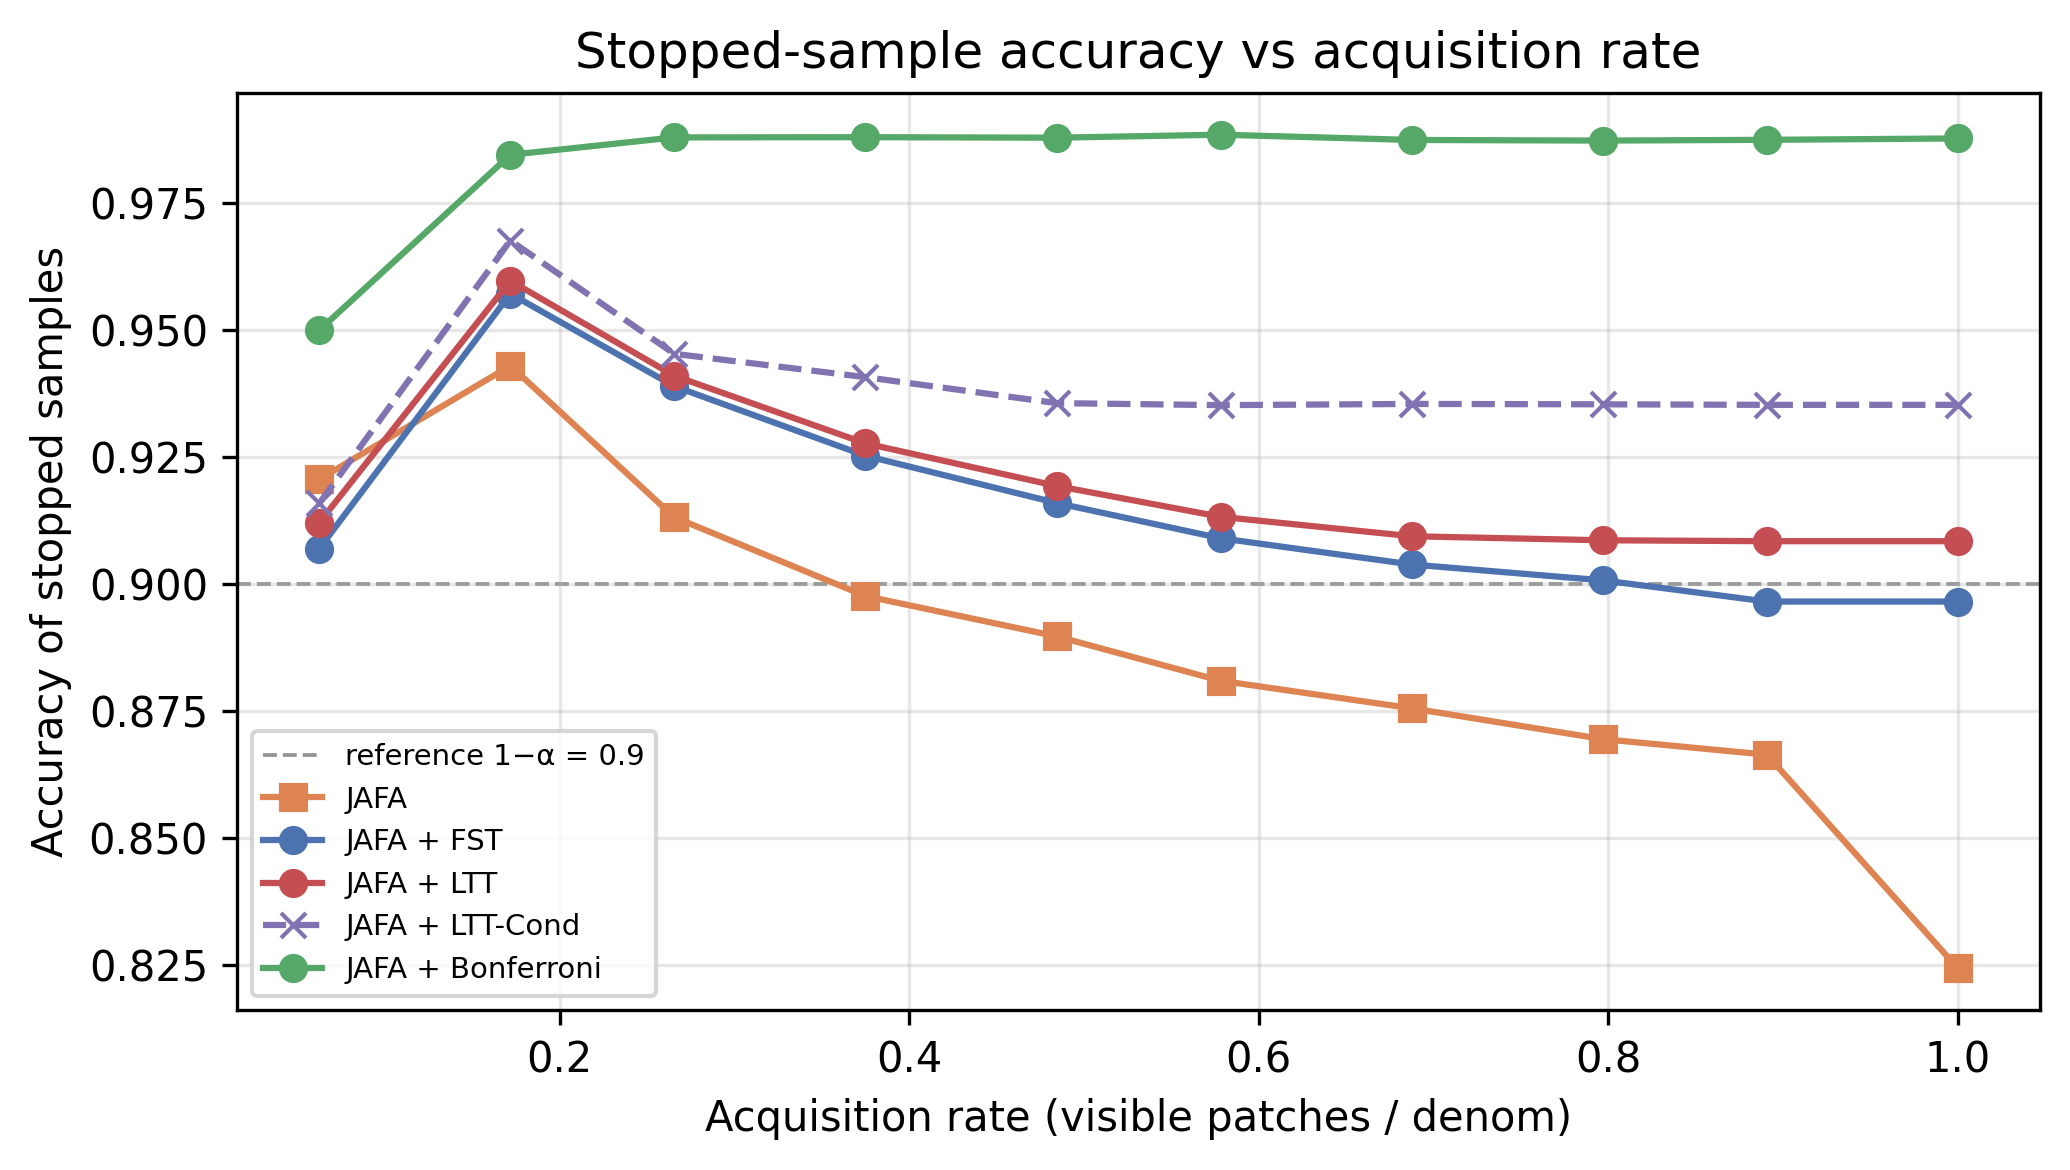
\includegraphics[width=\linewidth]{figures/compare_rl_jafa_stopped_accuracy_vs_rate_max_score_q_margin_max.png}
%         \caption*{(a) \textbf{CIFAR-10} : Accuracy among stopped samples against sampling rate}
%     \end{minipage}\hfill
%     \begin{minipage}{0.48\textwidth}
%         \centering
%         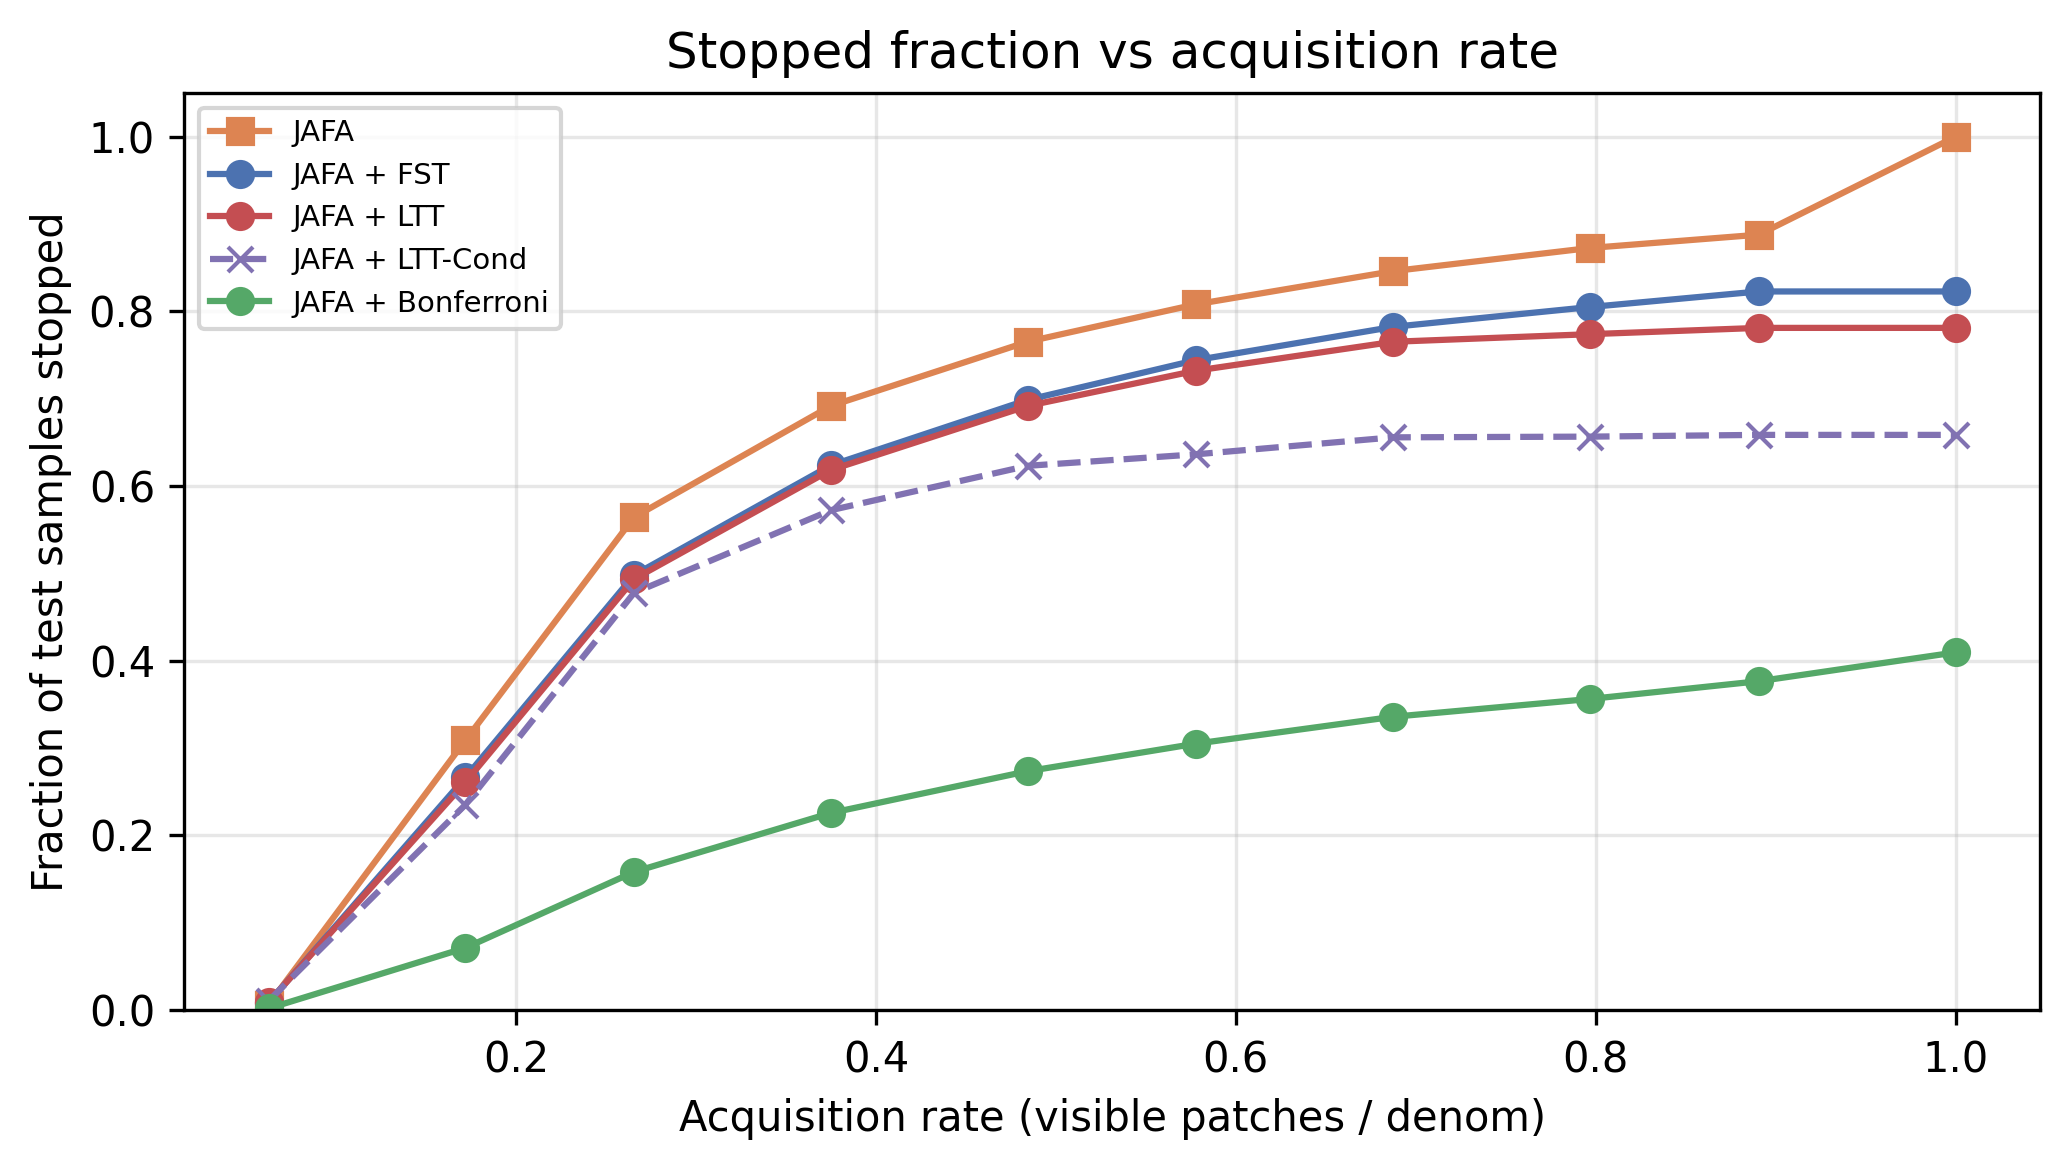
\includegraphics[width=\linewidth]{figures/compare_rl_jafa_stopped_vs_rate_max_score_q_margin_max.png}
%         \caption*{\textbf{CIFAR-10} : Fraction of stopped samples against sampling rate}
%     \end{minipage}
%     \caption{Complementing RL-based learned acquisition policies }
%     \label{fig:two-plots}
% \end{figure}

% \begin{figure}[ht]
%     \centering
%     \begin{minipage}{0.48\textwidth}
%         \centering
%         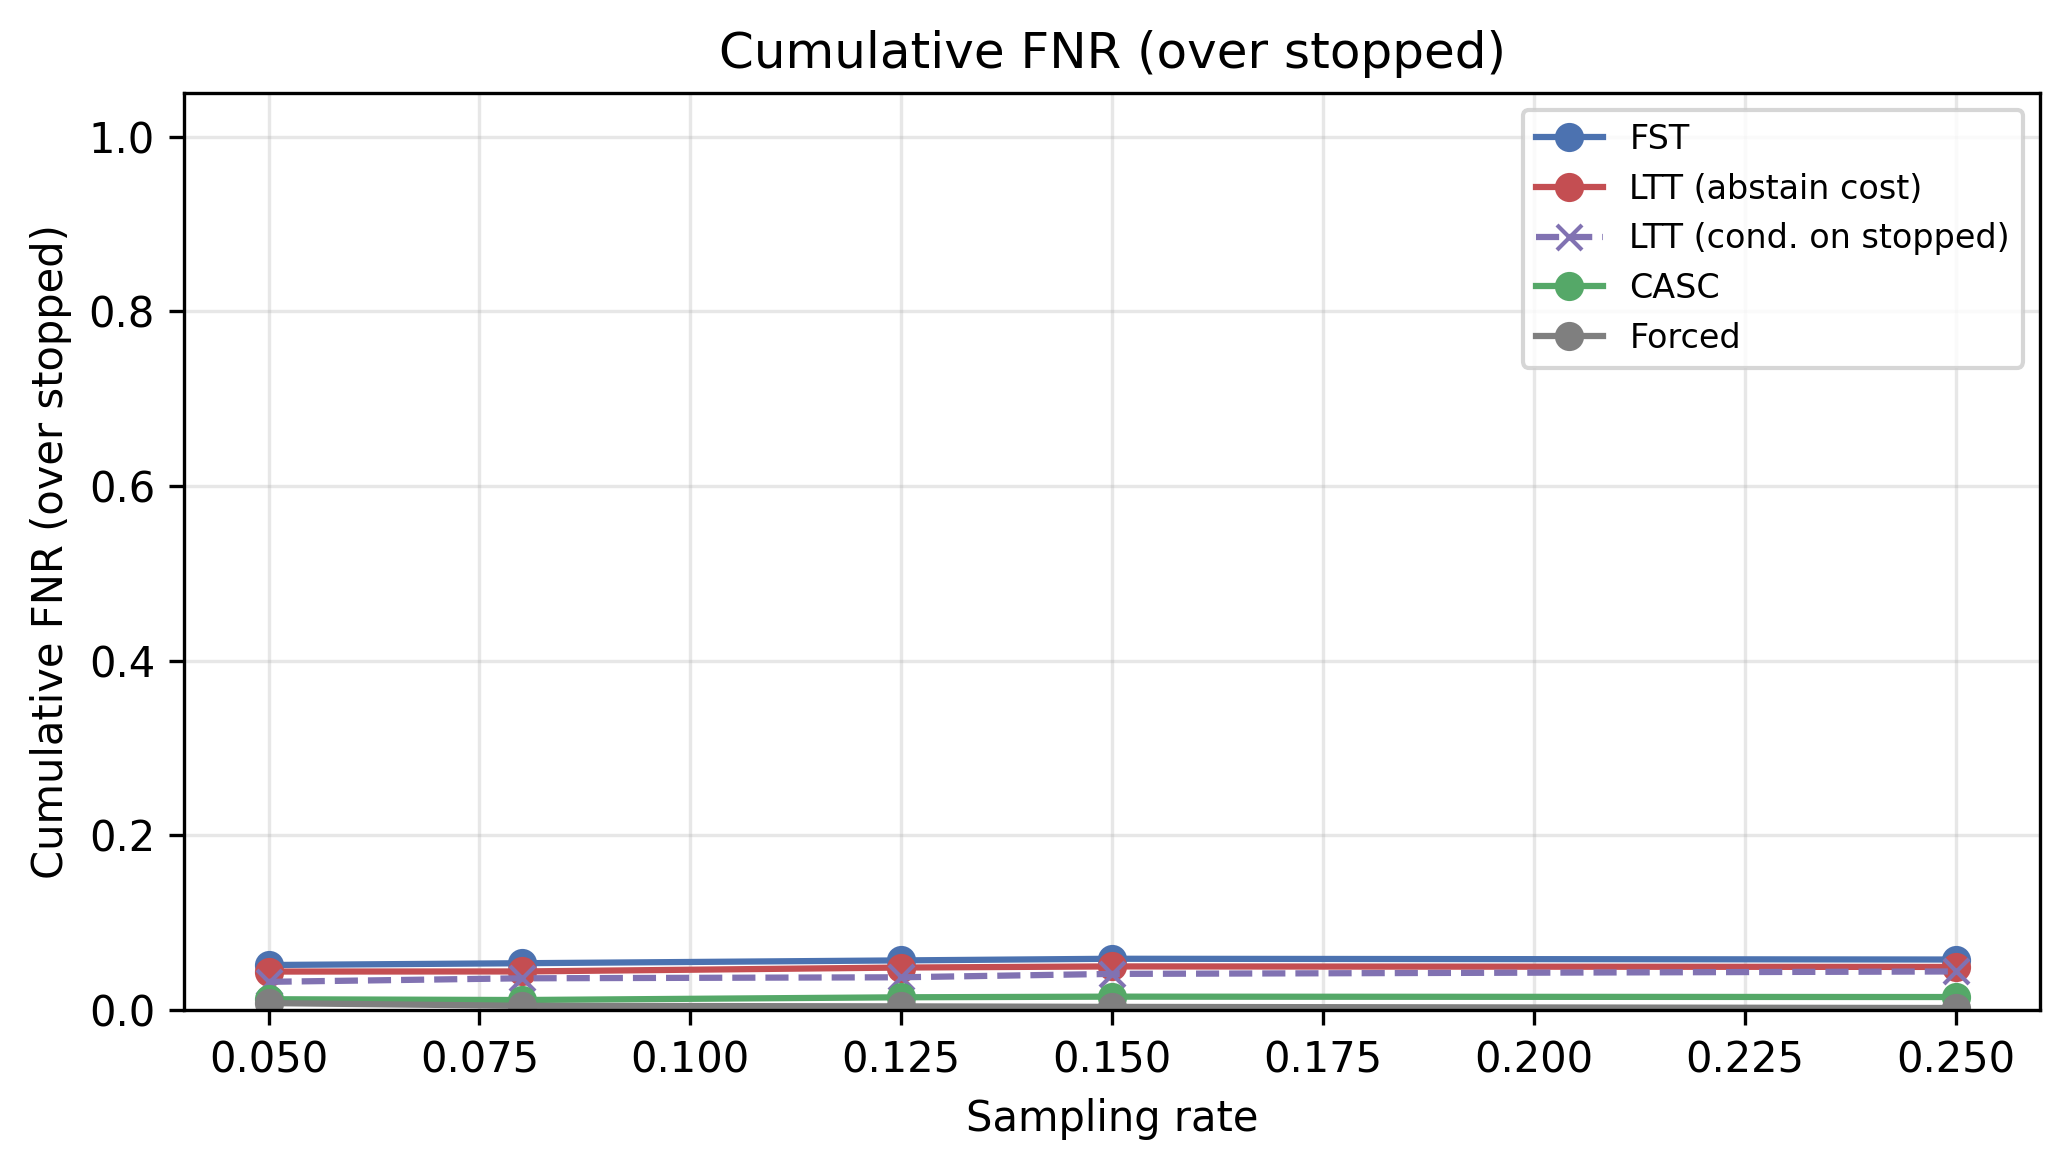
\includegraphics[width=\linewidth]{figures/knee_slice_compare_fnr_cumulative_vs_sampling_rate_knee_slice_fnr.png}
%         \caption*{(a) \textbf{FastMRI Knee Slices} : FNR among stopped samples against sampling rate}
%     \end{minipage}\hfill
%     \begin{minipage}{0.48\textwidth}
%         \centering
%         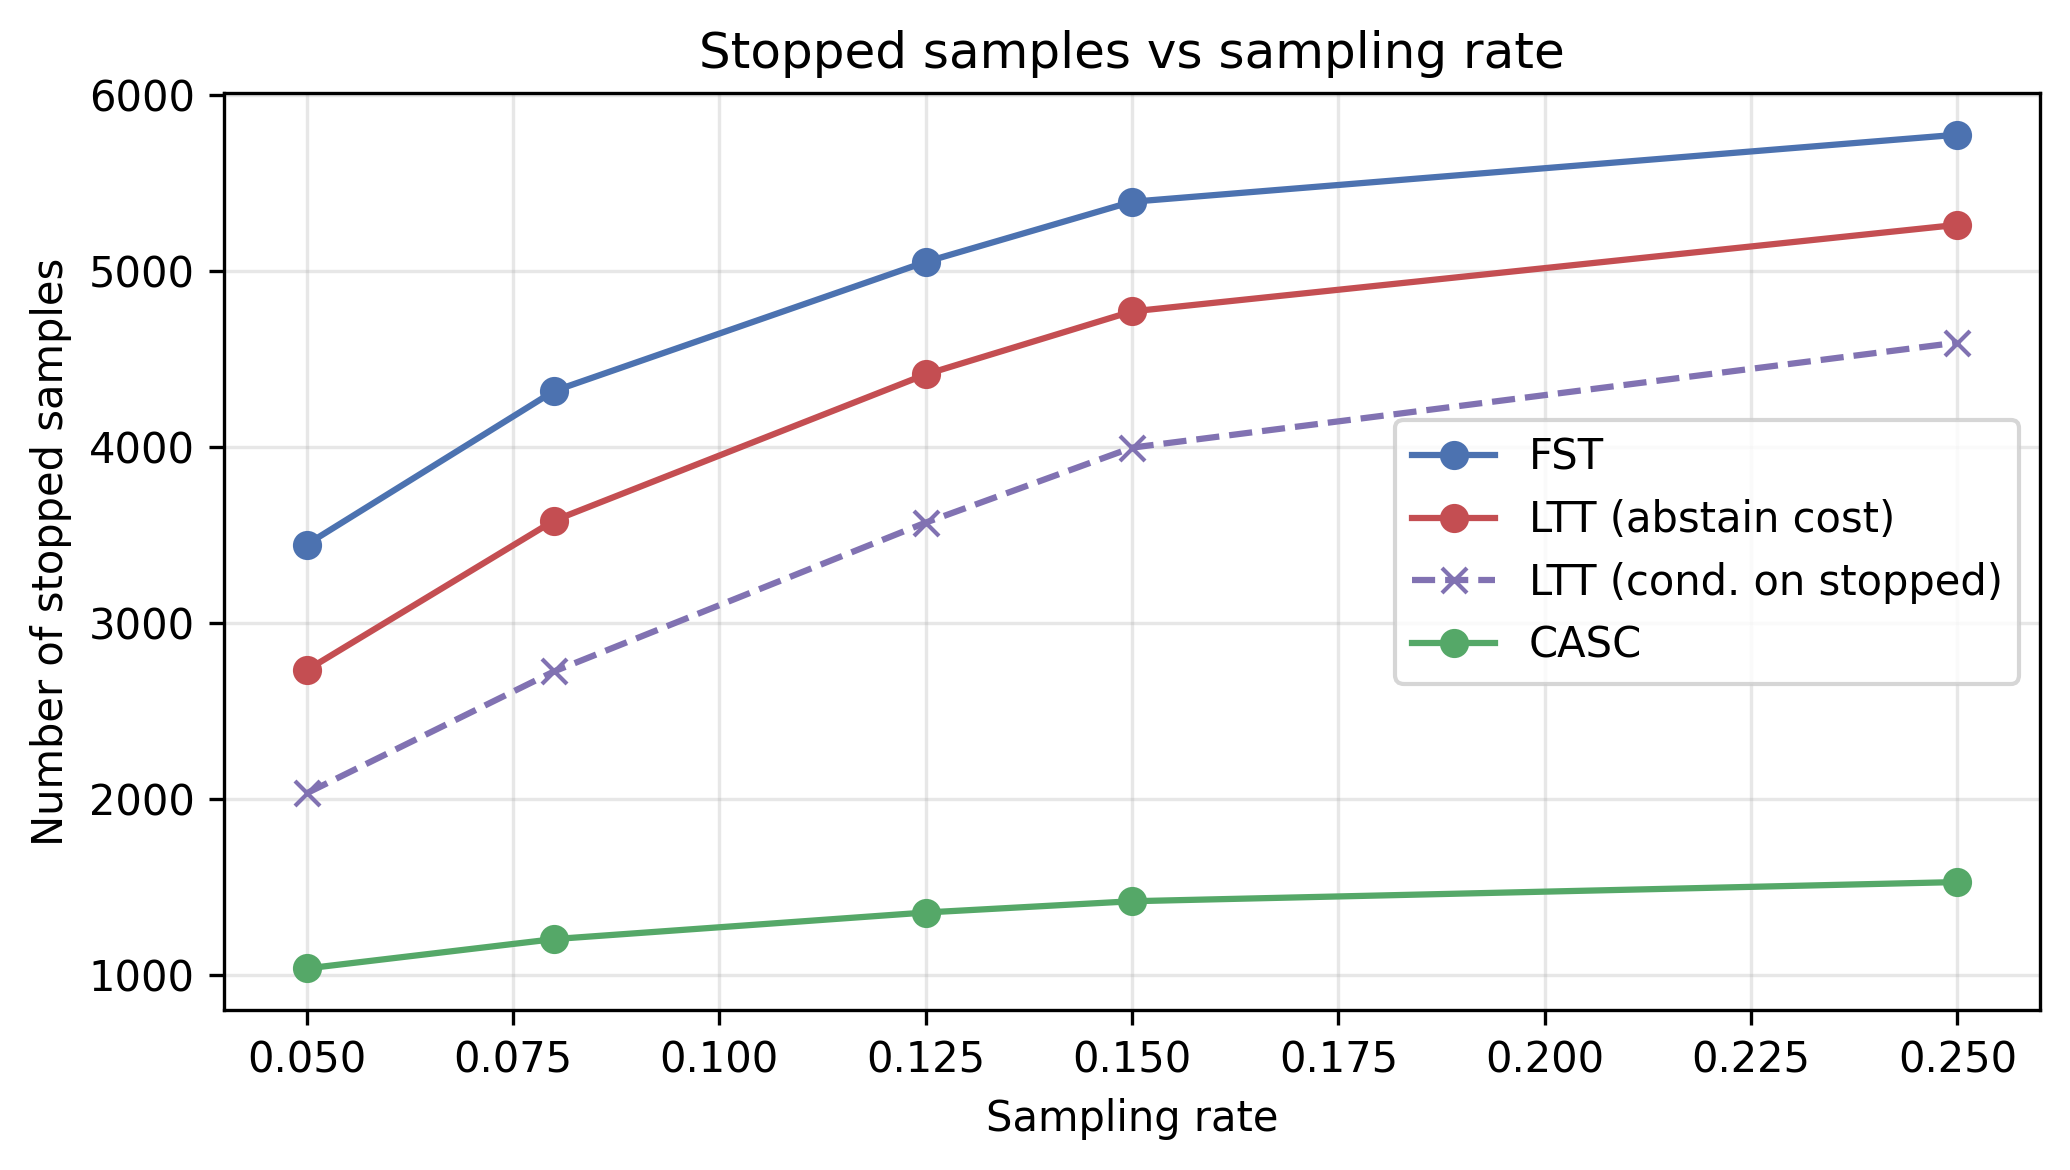
\includegraphics[width=\linewidth]{figures/knee_slice_compare_stopped_vs_sampling_rate_knee_slice_fnr.png}
%         \caption*{\textbf{FastMRI Knee Slices} : Fraction of stopped samples against sampling rate}
%     \end{minipage}
%     \caption{FastMRI Knee Slice-level Results}
%     \label{fig:two-plots}
% \end{figure}

% \begin{figure}[ht]
%     \centering
%     \begin{minipage}{0.48\textwidth}
%         \centering
%         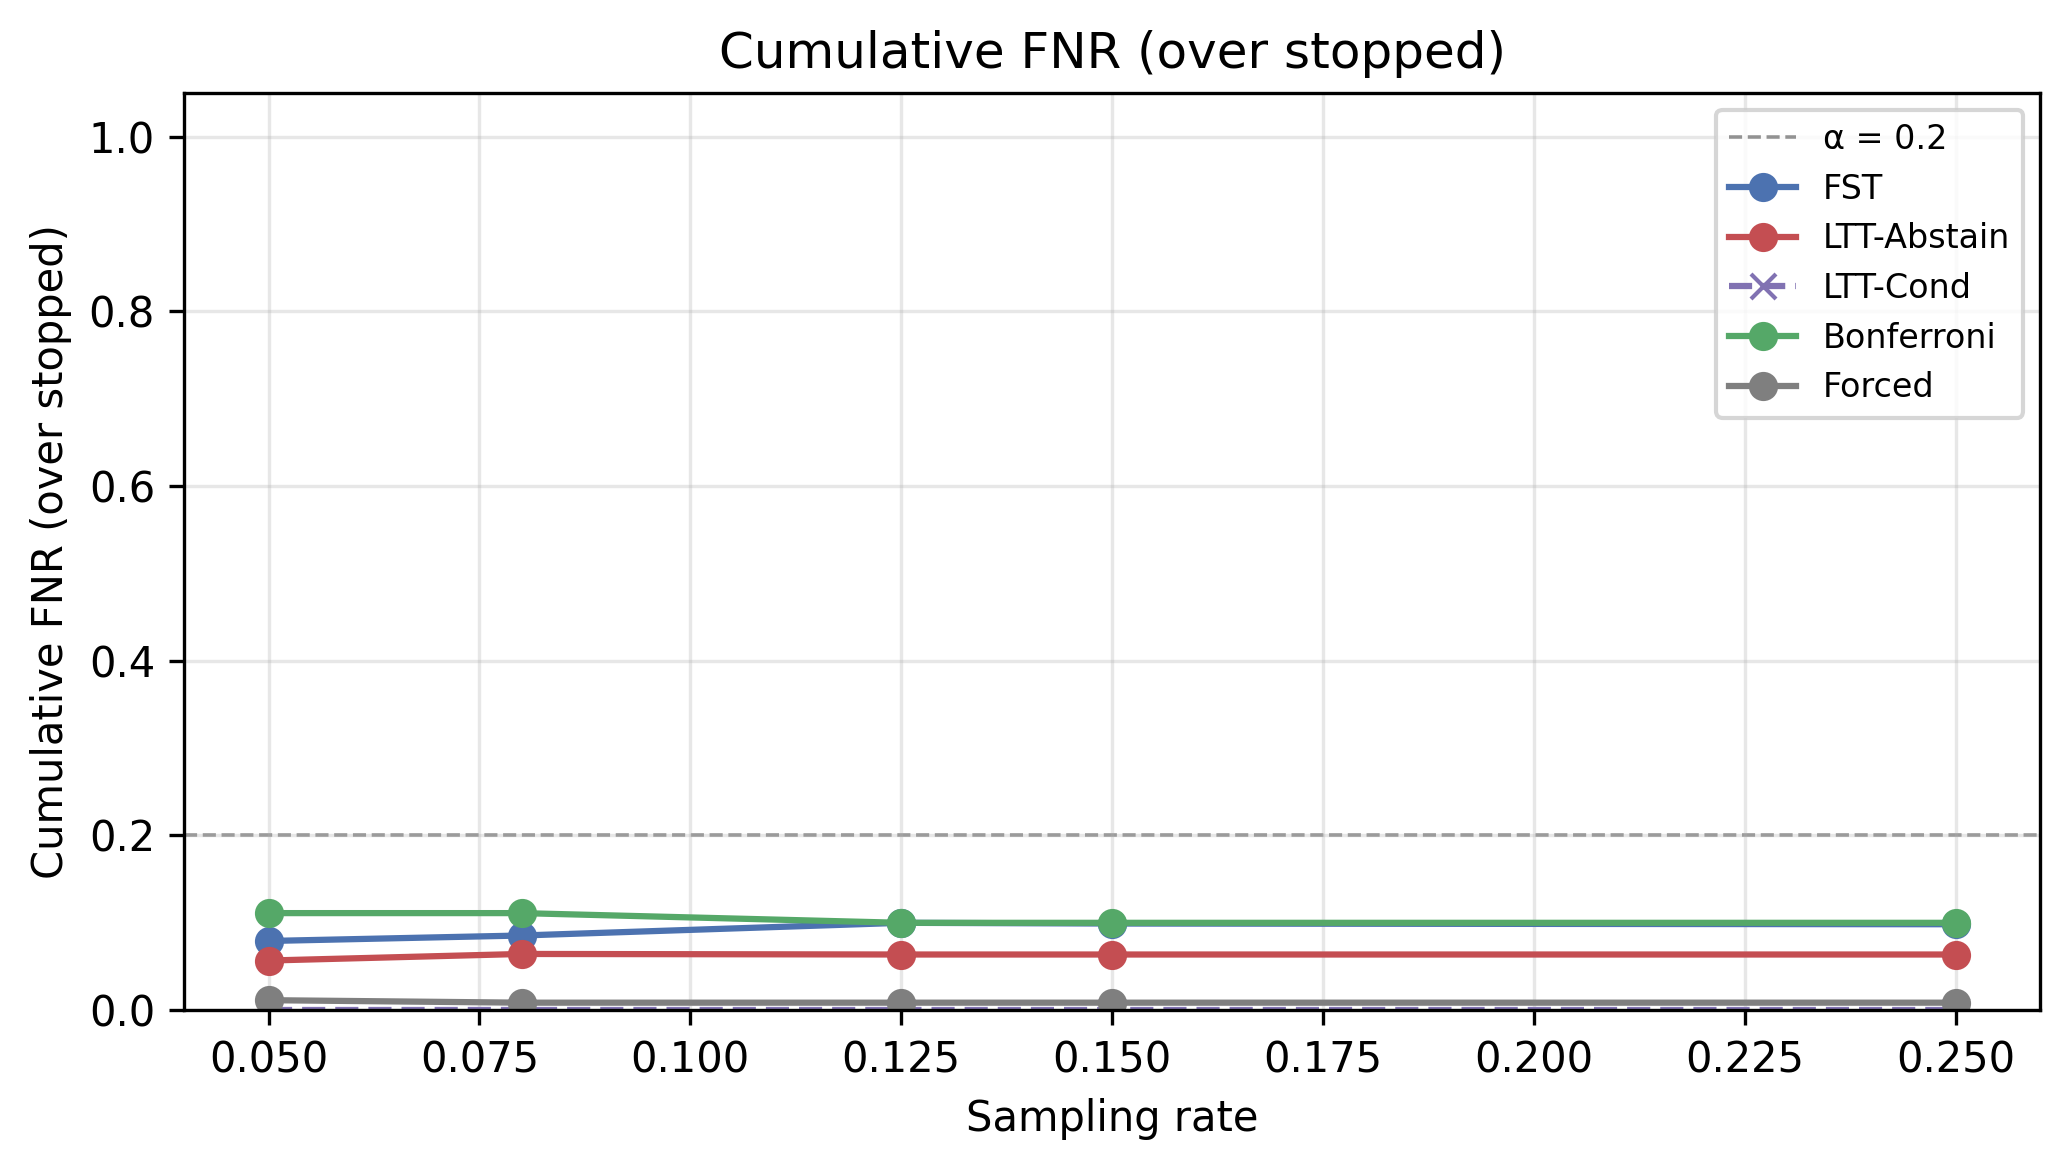
\includegraphics[width=\linewidth]{figures/knee_vol_asym_compare_fnr_cumulative_vs_sampling_rate_knee_vol_fnr_asym.png}
%         \caption*{(a) \textbf{FastMRI Knee Volumes} : Accuracy among stopped samples against sampling rate}
%     \end{minipage}\hfill
%     \begin{minipage}{0.48\textwidth}
%         \centering
%         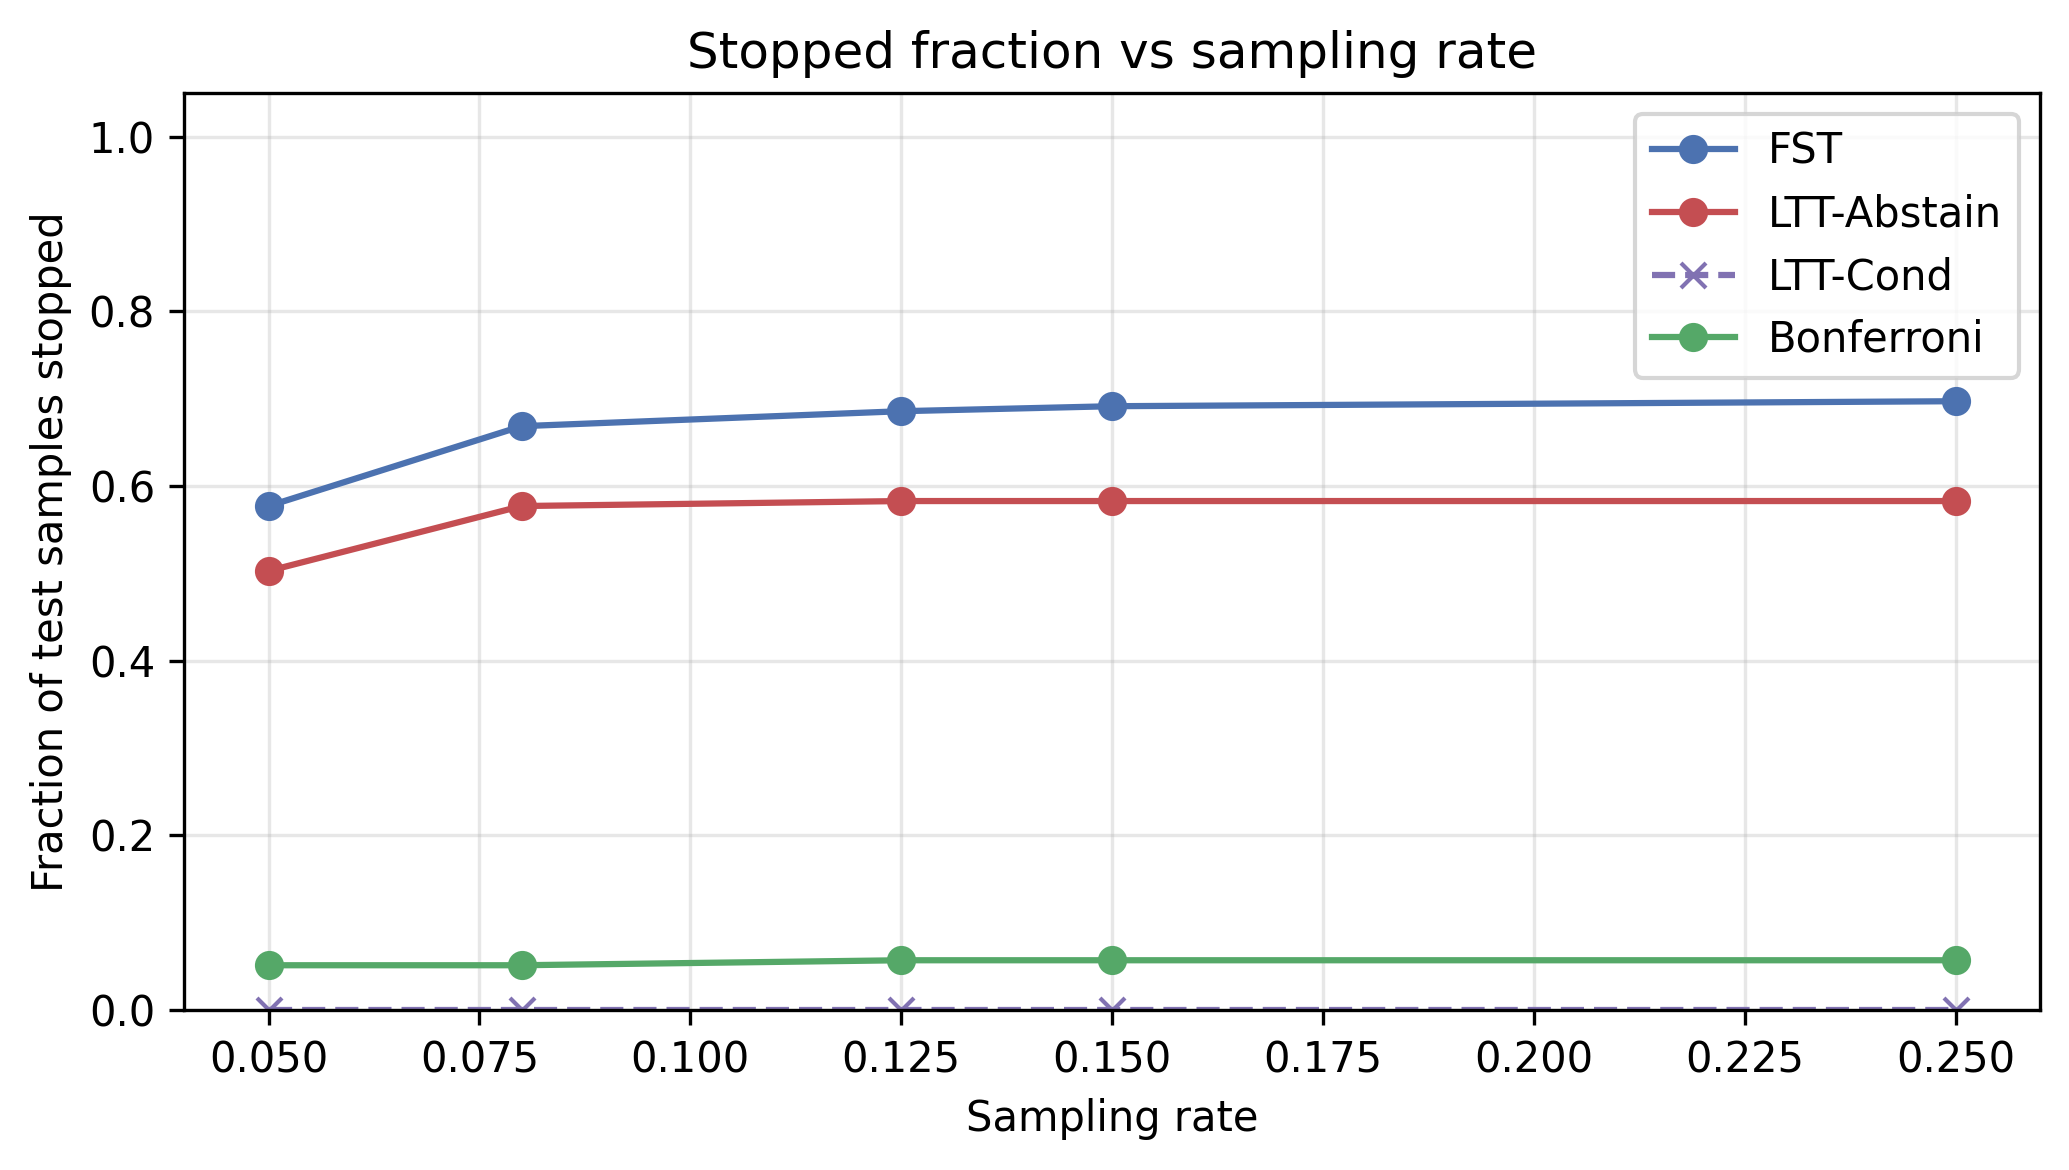
\includegraphics[width=\linewidth]{figures/knee_vol_asym_compare_stopped_vs_sampling_rate_knee_vol_fnr_asym.png}
%         \caption*{\textbf{FastMRI Knee Volumes} : Fraction of stopped samples against sampling rate}
%     \end{minipage}
%     \caption{FastMRI Knee Volume-Level Results}
%     \label{fig:two-plots}
% \end{figure}

% \begin{figure}[ht]
%     \centering
%     \begin{minipage}{0.48\textwidth}
%         \centering
%         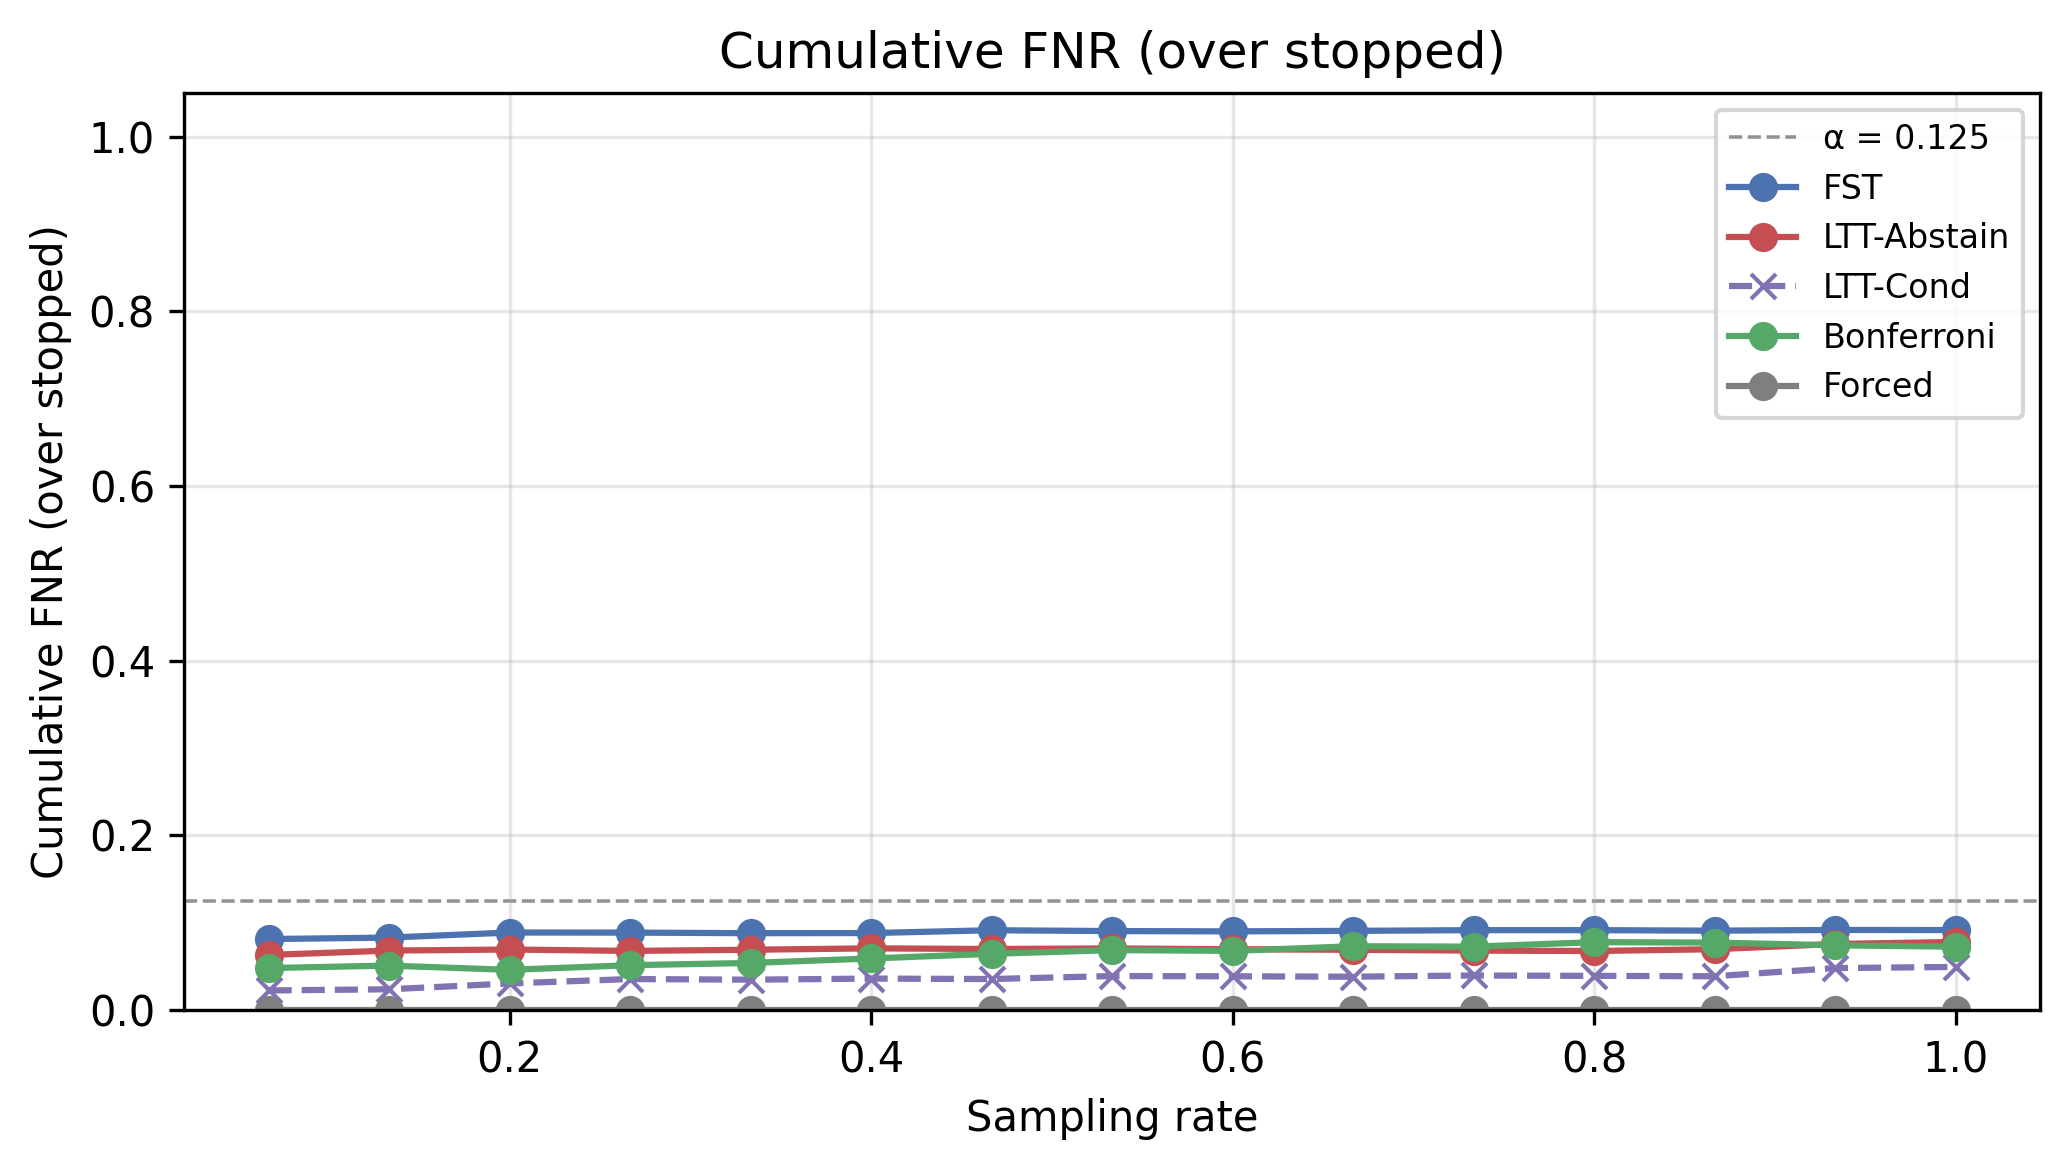
\includegraphics[width=\linewidth]{figures/prostate_asym_compare_fnr_cumulative_vs_sampling_rate_prostate_pirads_fnr_asym.png}
%         \caption*{(a) \textbf{Prostate} : Accuracy among stopped samples against sampling rate}
%     \end{minipage}\hfill
%     \begin{minipage}{0.48\textwidth}
%         \centering
%         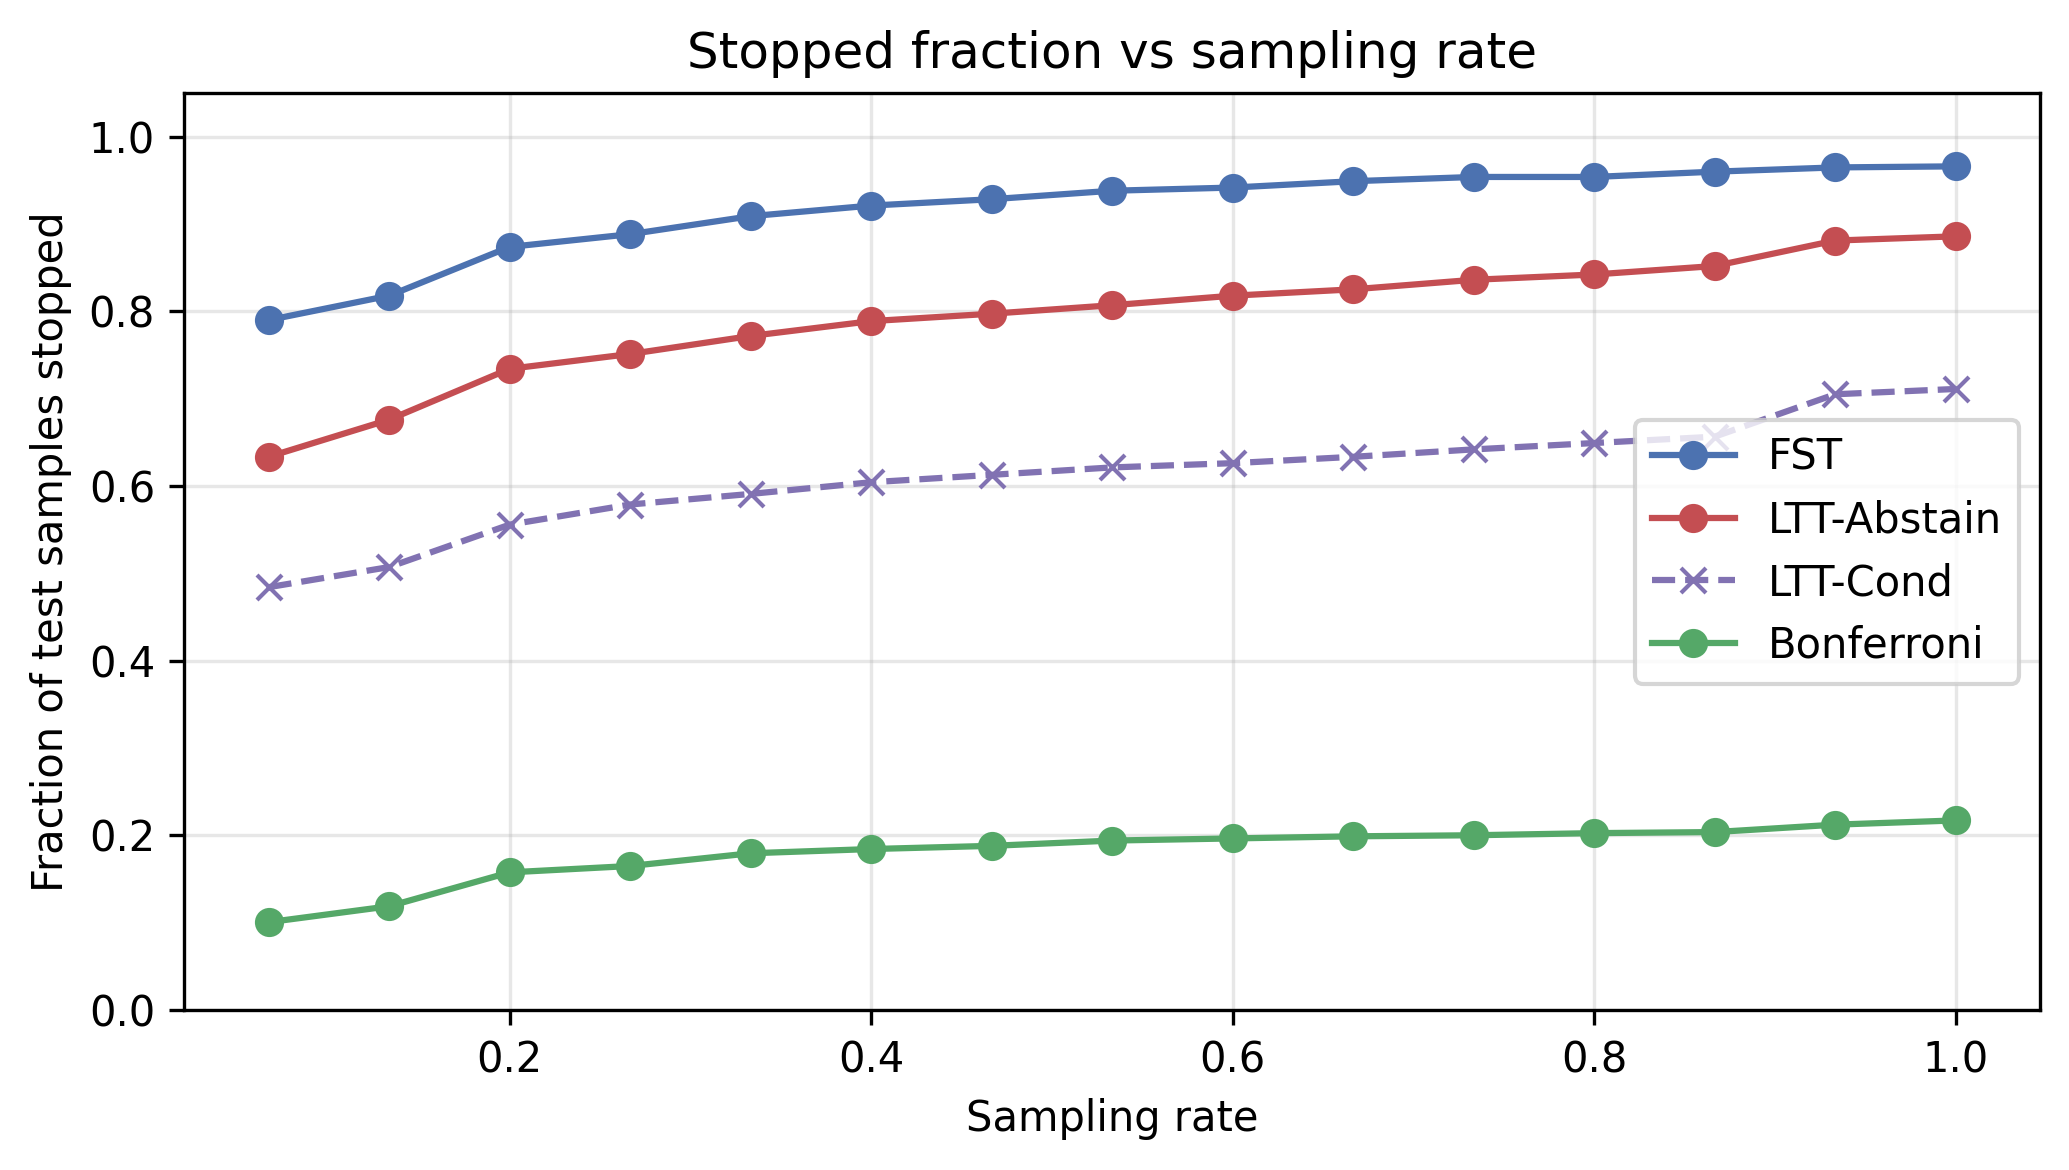
\includegraphics[width=\linewidth]{figures/prostate_asym_compare_stopped_vs_sampling_rate_prostate_pirads_fnr_asym.png}
%         \caption*{\textbf{Prostate} : Fraction of stopped samples against sampling rate}
%     \end{minipage}
%     \caption{FastMRI Prostate Results}
%     \label{fig:two-plots}
% \end{figure}

